\newcommand{\puttitle}{Milestone 5}
\documentclass{article}
\usepackage{geometry} % to change the page dimensions
\usepackage{graphicx}
\geometry{letterpaper} % or letterpaper (US) or a5paper or....
\geometry{margin=1in} % for example, change the margins to 2 inches all round

% Package for clickable TOC
\usepackage{hyperref}
\hypersetup{
    colorlinks,
    citecolor=black,
    filecolor=black,
    linkcolor=black,
    urlcolor=black
}

\usepackage{makeidx}
\makeindex
\usepackage[totoc=true]{idxlayout}
\newcommand{\createindex}[1]{#1\index{#1}}

\usepackage{glossaries}
\makeglossaries
% Changes from \section{<title>} to \subsection{<title>}
\setglossarysection{section}

\newcommand{\glossaryentry}[2]{\newglossaryentry{#1}{name={#1},description={#2}}}

% place glossary entries here
% ex: \glossaryentry{word}{description}
\glossaryentry{PostgreSQL}{open source object-relational database system}

\usepackage{pdfpages}
\usepackage{outlines}
\usepackage[parfill]{parskip} % to begin paragraphs with an empty line rather than an indent
\usepackage{multirow} %This is for making prettier tables and splitting columns and rows.
\usepackage{supertabular} %This is for making tables that extend over multiple pages
\usepackage{listings} %This is for listing source code
%\usepackage{tocbibind} %This is for including the bibliography in the table of contents.
\usepackage{appendix} %This gives more control over the appendix and how it appears in the table of contents.
\usepackage{tabularx} %This is to make stretchy columns in tables
\usepackage[fleqn]{amsmath} %AMS packages give more control over positioning and format of equations
\usepackage{amssymb}
\usepackage{amsthm}

\begin{document}
\begin{titlepage}
\begin{center}

\includegraphics[width=0.15\textwidth]{../images/rh}\\[1.0cm]
\textsc{\large Rose-Hulman Institute of Technology}\\[1.5cm]

\includegraphics[width=0.75\textwidth]{../images/pss}\\[1.0cm]
\textsc{\large{\puttitle}}\\[1.0cm]
\large Trey Cahill \hspace{0.2cm} Chris Gropp \hspace{0.2cm} Samad Jawaid \hspace{0.2cm} Kevin Risden
\vfill
\large \today
\end{center}
\end{titlepage}

\tableofcontents
\newpage

\section{Executive Summary}
This document's purpose is to detail the participant scheduling system proposed by the \index{Human-Computer Interaction Lab} Human-Computer Interaction Lab of Wisconsin-Madison. It is the fifth document describing this project, and contains interface designs constructed from the use cases of Milestone 2,the results of usability analysis on that interface, and planned changes based on this analysis. The project exists because the lab wishes to unify their schedule information and provide a simple, intuitive interface for prospective participants to sign up for experiments.

\section{Introduction}
The \index{Human-Computer Interaction Lab} at the University of Wisconsin-Madison wants a web-based system to better manage the scheduling of participants for their studies.  These studies range from one-on-one experiments to group interactions, and many of them involve the robot used by the lab.  Currently, each researcher arranges studies independently via email and is responsible for scheduling rooms, avoiding conflicts, and notifying participants of changes; unifying this information onto one system simplifies all of these tasks.  To the client, the most important benefit of a unified system is the ability for participants to easily browse all available experiments, which is not possible over email.  However, a variety of other functionality should be integrated into this utility to take advantage of the unity of information; most notable is recognizing room conflicts when scheduling studies, since the lab has only one robot and it cannot be moved.\cite{website:HCI}

Project information will be documented as follows:  Milestone 1 provides an overview of the project, from client background to key features and requirements.  Milestone 2 covers the behavior of the system, including use cases and data flow diagrams.  Milestone 3 details constraints, back-end requirements, and elaborates upon the user interface.  Testing and maintenance information can be found in Milestone 4.  Milestone 5 will include usability data and interface re-design related to such data.
\section{Client Background}
The client is the Human-Computer Interaction Lab at the University of Wisconsin-Madison. Their research focus is the on the way humans perceive computers, and how this perception influences their actions. The main goal is to learn about this interaction through making hypotheses, experimenting, analysing the data, and then publishing papers on the results.  They draw the participants for their experiments from a wide range of people, usually ranging from 18-65 years of age and from diverse technical backgrounds.  As such, any system they use must be designed for all levels of technical competency.
\section{Current System}
Each researcher has their own method of handling participant scheduling. For most the current system is to have the participants email the individual researcher and then that researcher records the time slot in some sort of excel spreadsheet. Other researchers have tried Google Calendar appointment slots; while this is a better system, not everyone uses it and the client believes it is too complex for most participants and some researchers.  Addressing the lack of unified data and superfluous effort on the part of the participants is the primary goal of the project.
\section{Product Overview}
This section provides a high-level view of the product capabilities, interfaces to other applications, and system configurations.

\subsection{Product perspective}
The participant scheduling system will be a new product. It will be used to schedule experiments and participants in the Human-Computer Interaction Lab at the University of Wisconsin-Madison. The product is independent and totally self-contained, besides a few external software packages; it is not a component of a larger system.

\subsection{Elevator Statement}
For the researchers in the Human-Computer Interaction Lab at the University of Wisconsin-Madison who currently schedule experiments and participants with rudimentary tools such as pencil and paper, email, or Google Calendar, the participant scheduling system will be a web application that will streamline the lab's scheduling process. Unlike current solutions, this application will be the same for every researcher, so it will also be easier for participants to be a part of multiple experiments.

\subsection{Summary of Capabilities}
Here are the major benefits and features the product will provide.
\begin{table}[!h]
    \begin{tabular}{|l|l|}
        \hline
        Customer Benefit & Supporting Feature \\ \hline
        List of participants for an experiment & Reports \\ \hline
        Room availability (avoid conflicts) & Overall lab schedule \\ \hline
        Simple sign up & Intuitive user interface \\ \hline
        Track all experiments & Experiments manager \\ \hline
        Access from anywhere at any time & Web application \\ \hline
    \end{tabular}
\end{table}
\subsection{Assumptions and Dependencies}
\begin{itemize}
\item The participant scheduling system will be a web application.
\item The server has the necessary operating system and software.
\item There is no integration with any other system.
\item There is no import of existing data.
\end{itemize}
\subsection{Rough Estimate of the Cost}
There is no monetary cost for this project, because the software development, as part of a college class, is free. Similarily, all software used is open-source. Furthermore, the client will be provided with free servers through the University of Wisconsin-Madison for the finished product. The client will perform maintenance and management on their own.

\clearpage
\section{Features}
\begin{table}[!h]\footnotesize
    \begin{tabular}{|p{.5cm}|p{2.5cm}|c|c|p{1.25cm}|p{1cm}|p{1.25cm}|p{1cm}|p{3.75cm}|}
        \hline
         ID & Feature & Status & Priority & Effort & Risk & Stability & Target Release & Reason \\
        \hline
        1 & Browse Experiment & Approved & Critical & Medium & Medium & Medium & 1st & Lets experiments be advertised better and to display the experiments \\
        \hline
        2 & Persistent Experiment Storage & Approved & Critical & Medium & Low & High & 1st & Store experiment for the data to be web based. \\
        \hline
        3 & Levels of Authentication & Approved & Useful & Medium & High & Medium & 3rd & Have levels of administrators, workers and participants in order to control privacy issues and other sensitive data \\
        \hline
        4 & Participant Schedule Experiment & Approved & Critical & Medium & Medium & Medium & 1st & Participant can schedule experiment slot \\
        \hline
        5 & Filter Experiments & Approved & Useful & Medium & Low & High & 2nd & Filter the experiments when browsing according to Time, Date, Payment, etc. \\
        \hline
        6 & Experiment Participants & Approved & Important & Low & Low & High & 2nd & View all of the participants by admins and workers only of individual experiments \\
        \hline
        7 & Cancel Experiment Appointment & Approved & Useful & Medium & Medium & Medium & 3rd & Cancel participant scheduled appointment \\
        \hline
        8 & Add Experiment & Approved & Important & Medium & Medium & Medium & 2nd & Add experiment from admins view \\
        \hline
        9 & Modify Experiment & Approved & Important & Medium & Medium & Medium & 2nd & Modify or Edit experiment from admins view \\
        \hline
        10 & Notify Participant when Creating Appointment & Approved & Useful & Medium & Low & High & 4th & Send an email reminding participants of participation in an experiment \\
        \hline
        11 & Notify Participant Appointment Reminder & Approved & Useful & Medium & Low & High & 4th & Send an email or text reminding participants for their experiments \\
        \hline
         12 & Notify Participant Appointment Cancellation Reminder & Approved & Useful & Medium & Low & High & 4th & Send an email or text reminding/telling participants of cancellation of their experiments \\
        \hline
        13 & Export Experiment Participant List & Approved & Useful & High & Low & High & 4th & Reports on experiments scheduled with an option for Individual experiments reports \\
        \hline
        14 & All Experiments Calendar & Approved & Useful & Medium & Low & Low & 4th & Have an overall schedule viewer \\
        \hline
        15 & Remove Experiments & Approved & Important & Low & Low & High & 4th & Allow for workers or administrators to remove schedules \\
        \hline
        16 & Tracking of Consent Payment Forms & Rejected & Useful & Medium & Low & Medium & N/A & Allow for workers to check off participants when filling out consent/payment forms \\
        \hline
        17 & User Report & Rejected & Useful & Medium & Low & Medium & N/A & Allow participants to have a report on new experiments \\
        \hline
        18 & Accounts & Approved & Critical & High & Low & Medium & N/A & Accounts for participant \\
        \hline
        19 & Prevent Scheduling Conflicts (Participant) & Approved & Useful & High & Low & Medium & N/A & Prevent participants from scheduling 2 experiments at the same time \\
        \hline
        20 & Prevent Scheduling Conflicts (Administrator) & Approved & Useful & High & Low & Medium & N/A & Prevent 2 rooms from being scheduled at the same time \\
        \hline
        21 & Install Scripts & Proposed & Useful & High & Low & Low & TBD & Install scripts for installation \\
        \hline
        22 & Documentation for Maintenance and User & Approved & Useful & High & High & Low & Ongoing & Documentation \\
        \hline
    \end{tabular}
\end{table}
\clearpage
The \textbf{Browse Experiments} feature and \textbf{Persistent Experiment Storage} both had a Priority of Critical since they both must be implemented for even a very basic version of the scheduling System.  The effort on both was a medium as with a team of two, there would be a manageable amount of work.  \textbf{Browse Experiments} has a stability of medium since it is up for change upon the client seeing the UI.  \textbf{Persistent Experiment Storage} has a stability of high since once implemented has little chance of being changed.

\textbf{Participant Schedule Experiment} has a priority of critical since the participants must be able to sign themselves up for an experiment for the project to be successful.  Again, the effort is medium since with two people the work would be manageable.  The risk is high on this feature, since the success of the project has a dependence on the feature.  The stability would be medium since the steps are unlikely to change, but the UI could easily change.

\textbf{Levels of Authentication} is a useful priority because it would not be necessary for there to be an actual Admin since the users trust each other, but this would be a nice feature.  The effort and stability are medium since the feature may change some, but only smaller parts of the feature, while still being a very manageable task.

\textbf{Filter Experiments} has a priority of useful, since it might only apply to users in certain situations.  \textbf{Filer Experiments} and \textbf{Experiment Participants} have a low risk, since the project does not depend on their success.  They both also have a stability of high, since changes are unlikely to happen.  The effort on \textbf{Filter Experiments} is medium, since there are some areas of the feature, such as what to filter by, that have not been established.  The  effort on \textbf{Experiment Participants} is low since a simple SQL query will do most of the job.

\textbf{Cancel Experiment Appointment}, \textbf{Modify Experiment}, and \textbf{Add Experiment} get and effort of Medium, since most deal with SQL and some logic on the back end.  They also have a risk of medium, since a mistake while implementing these features could create a difficult to find bug elsewhere.  The stability is medium, since parts of the database could change slightly.

\textbf{Notify Participant When Creating Appointment}, \textbf{Notify Participant Appointment Reminder}, and \textbf{Notify Participant Appointment Cancellation Reminder} all have a priority of useful since they would be nice to have, but are not vital to the projects success.  They all have an effort of medium since they involve a persons email, but could be reduced to low, depending of the framework used.  Their risk is low, since a failure here creates no problems else where in the project, nor does a mistake spread else where in the project.  The stability is high on these since they are unlikely to change.

\textbf{User Information Form} has a priority of critical since the user must enter their information when scheduling for an experiment.  The effort is low since this will be a simple UI, but the Risk is High since the User information must be stored for the experiment.  The stability is high since all that is needed is name, phone number, and email.  

\textbf{Export Experiment Participant List} is a useful feature, that has a high effort due to formatting of the report.  The risk is low though, since the feature is not critical in the release of the product.  Stability is high due to the feature being very specific.

An \textbf{All Experiments Calendar} would be useful for the future participants.  The effort is medium because it would be an extension of the \textbf{Browse Experiments} feature.

\textbf{Remove Experiments} has a priority of Important, since, although rare, experiments may be cancelled. The effort is low since most of it will be taken care with an SQL query.  Also, a stability of high is given because of  how specific the feature is described.

\textbf{Accounts}, \textbf{Prevent Scheduling Confilicts for the Participant}, and \textbf{Prevent Scheduling Conflicts for the Administrator} all have a priority of useful, except for \textbf{Accounts} which Critical, since the other two features mentioned rely upon the \textbf{Accounts} along with cancellation of the experiment slots.  The effort is high for all the features due to the logic needed when implementing the features.  

\textbf{Tracking of Constent Payment Forms} and \textbf{User Report} have all been rejected, since the client does not need theses features.

\textbf{Documentation} and \textbf{Install scripts} are both useful priority.  The effort will be high, since there is complexity associated with the Install scripts and Documentation is difficult to keep up to date.  The stability would be low since the definition could change.

Items 1, 8, 15, 18, and 21 will be assigned to Kevin Risden.  Items 3, 4, 10, 11, and 12 will be assigned to Samad Jawid.  Items 6, 9,14 and 20  will be assigned to Chris Gropp.  Items 2, 5, 7, 13 and 19 will be assigned to Trey Cahill.  The entire team will work on item 22.

% Start - Milestone 5 specific parts
\section{Usability Report}
\subsection{Process}
In order to conduct the usability study, our team used the human computer interaction experts at the University of Wisconsin-Madison HCI Lab. Our client contacted 5 experts and they reviewed our prototype system. Before the experts could review our system, they had to agree to an Informed Consent Form that is included below. A list of tasks was then provided to the experts with instructions to fill out a questionnaire on Google Documents. The questionnaire included the Informed Consent Form at the top of the form and by submitting the questionnaire the experts were agreeing to the terms of the Informed Consent Form. The specific instructions given to the experts are included below as well. Once the experts had completed the tasks, they filled out the questionnaire here \url{https://docs.google.com/spreadsheet/viewform?formkey=dExyUjl2cGJiMUlfb0dfMkFNT1k1UEE6MQ} and the questions have been copied below. This process proved to be useful since we did not have to find a common meeting time for everyone and the experts could complete the tasks on his or her own time.

\subsubsection{Informed Consent Form}
Please read this informed consent document carefully before you decide to participate in this study.

The purpose of this study is to analyze and test the design of the proposed Participant Scheduling System for use at the Human-Computer Interaction Lab at the University of Wisconsin in Madison (henceforth HCI lab).

This study is being conducted by Trey Cahill, Chris Gropp, Samad Jawaid, and Kevin Risden, with additional support from Sriram Mohan, Jimmy Theis, and Allie Terrell (henceforth the study organizers). No other persons or agencies will assist in this study or be allowed access to any identifying information.

This study is confidential; your name and specific responses will not be available to anyone outside of the study organizers. Only aggregate information will be available to the general public, and your name will not be released in any capacity (as part of a list or otherwise) to anyone outside of the study organizers.

Your specific responses and any identifying information will be destroyed no later than June 2012, even amongst the records of the study organizers.

Your participation in this study is entirely voluntary. You may refuse to answer any questions posed, and may choose to stop participating at any time.

If you have questions about the study, please contact Kevin Risden by email at risdenkj@rose-hulman.edu

Your completion and submission of the questionnaire indicates your consent to participate in this study under the terms stated above.

\subsubsection{Expert Instructions}
Thanks so much for agreeing to help out with this usability study. As you saw in my previous email, this is for the participant scheduling system for the lab and is being completed as part of a class project by a team of students from my undergraduate school. Kevin Risden (who is heading the team working on this) is CCed on this email - please feel free to email him with any questions (CC me), or if you have further comments after completing the study.

The study should take about 30 minutes to complete - instructions are below this message. Note that there is a feedback form as well via Google Docs. Since this is part of a class, the team needs your responses by Thursday morning so they can complete their milestone. Additionally, I will be out of town all day Thursday. I've asked Kevin to send out a reminder email if he doesn't have all of the responses by then.

Keep in mind that this is a prototype - their winter quarter will be spent developing the working system. So, provide constructive feedback for the team, particularly regarding the design and functionality.

Prototype: http://pss.csse.rose-hulman.edu/

Below is a provided username and password to use to login to the system.\\
Username: aterrell\\
Password: temp123

Before attempting to complete the tasks below, spend a few minutes exploring the system to gain an understanding of it.

As a HCI Lab Researcher, here is the list of tasks to complete:
\begin{itemize}
\item Login
\item Add Experiment
\item Modify Experiment
\item Experiment Time and Date Range
\item Delete Experiment
\end{itemize}

Please complete a feedback form at https://docs.google.com/spreadsheet/viewform?formkey=dExyUjl2cGJiMUlfb0dfMkFNT1k1UEE6MQ as you proceed through the tasks.

Limitations:\\
Signup will not work due to verification emails not being allowed outside the Rose-Hulman Institute of Technology firewall.

\subsubsection{Questionnaire}
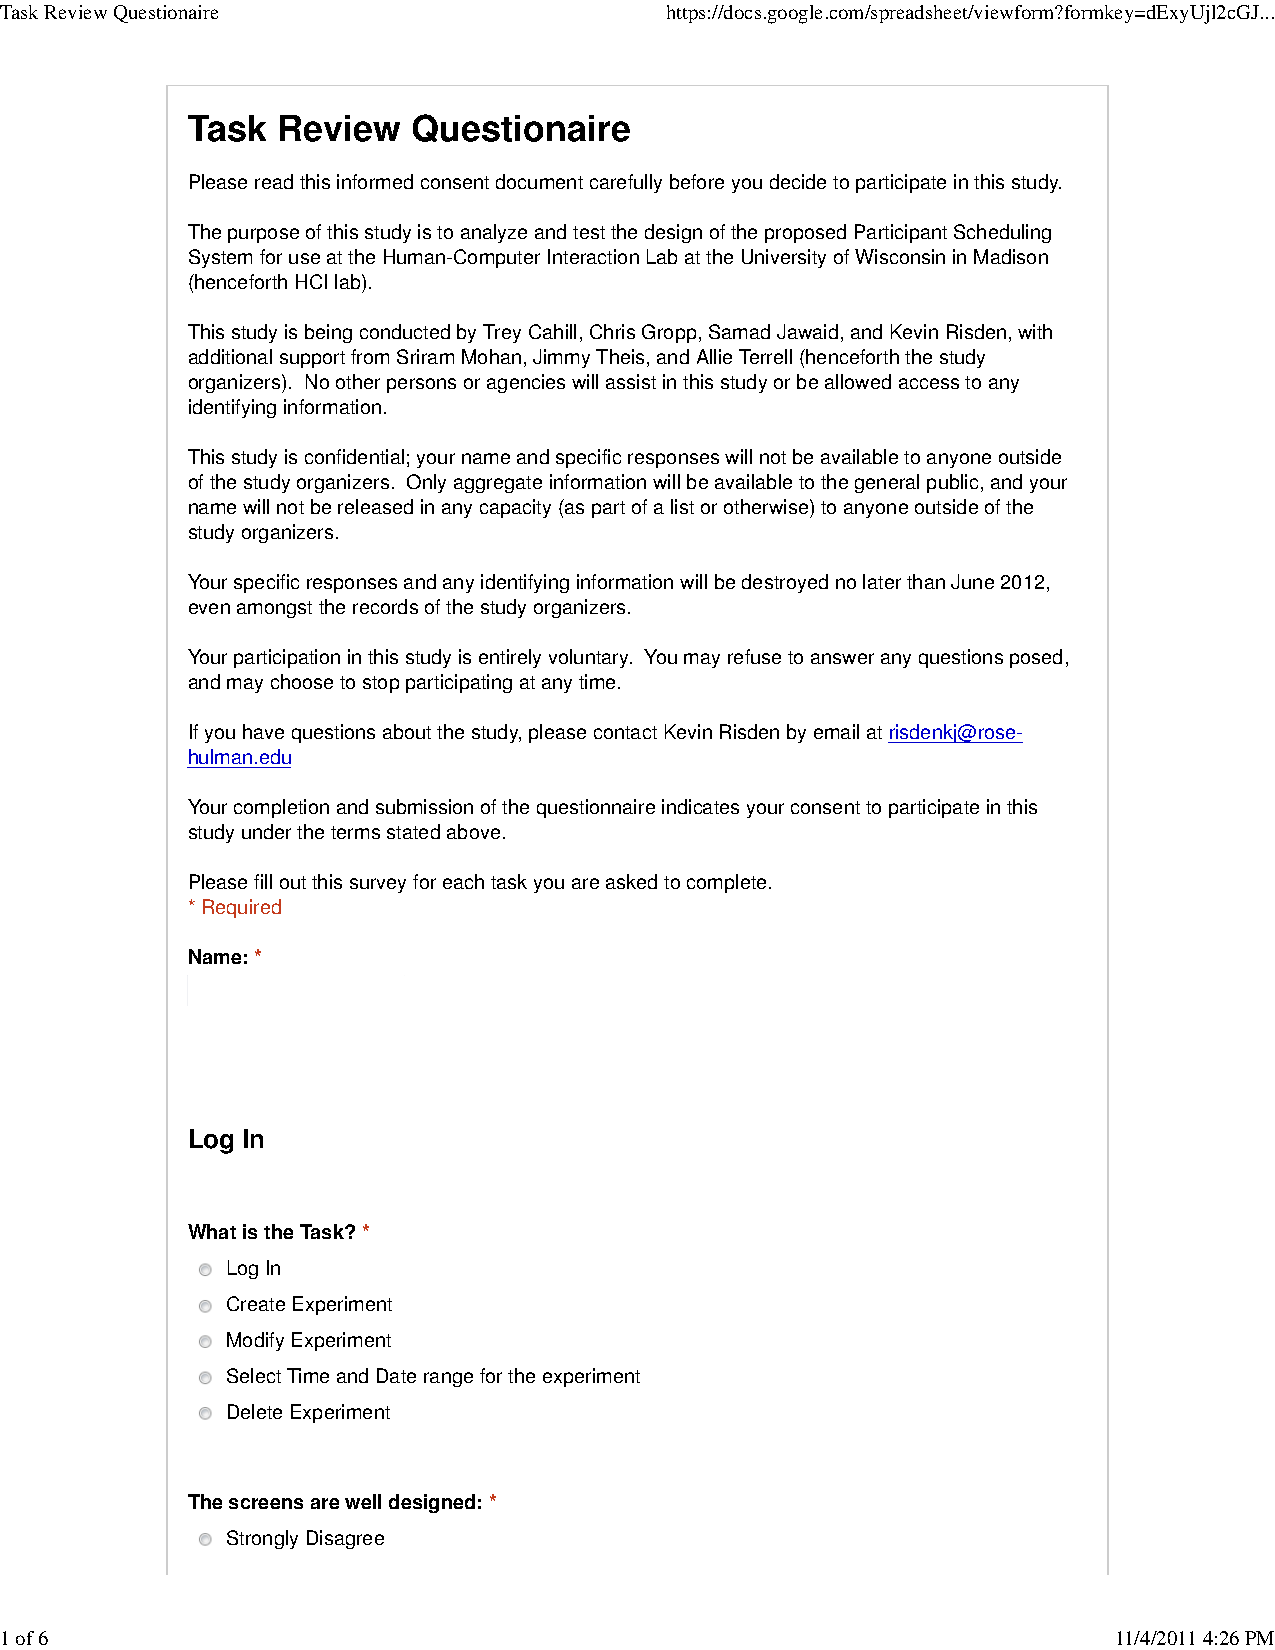
\includepdf[pages=1-,pagecommand={}]{../other/google_docs_questionnaire}

\subsection{Analysis}
Using the Google Documents form and corresponding spreadsheet provided a convenient way to aggregate the data and analyse it. The raw data was downloaded from Google Docs in Excel format and then the analysis of each task was done following the general structure outlined here:
\begin{itemize}
\item A bar chart showing the number of each type of response for how well the screen was designed.
\item The answers for the how well screen(s) were designed question were given a numerical value. Strongly disagree was given a 1, disagree a 2, neutral a 3, agree a 4, and strongly agree a 5. 
\item These scores were averaged to give an overall score for how well each task was designed in terms of the screens and displayed in a table.
\item Common themes for the two open ended questions were identified.
\end{itemize}
The three open ended questions at the end of the questionnaire relating to the overall feel of the system were each analysed for common themes. Based on the feedback from each participant, follow-up questions were generated in order to gain more specific information.

\subsubsection{Login}

\subsubsection{Add Experiment}

\subsubsection{Modify Experiment}

\subsubsection{Experiment Time and Date Range}

\subsubsection{Delete Experiment}


\subsection{Findings}
The analysis of the usability study provided some results that were expected due to the level of the prototype, but also some results that were unexpected. Overall findings are listed first followed by the findings broken out into the tasks the experts completed.

\subsubsection{Overall}


\subsubsection{Login}
The overall sentiment showed that the experts liked the simplicity of the home page and login page. The other suggestion was that the home page should provide information about the lab, which is planned for a later version when the experiments are displayed on the home page for participants to choose from. With the overall average rating being a 3.2, the experts were close to neutral due to the lack of content on the home page, but this was planned to be changed when more of the system is implemented.

\subsubsection{Add Experiment}
The comments for the Add Experiment question suggested that the division of creating an experiment and the time slots separately was a bad design. This should be integrated into one screen since the two activities are related. The ability to add rooms, qualifications, and researchers while creating an experiment is a feature that was missing from the initial prototype but is on the radar to be completed in the next revision. This hurt the usability since the experts could not create a new room or add a qualification. One comment related to not knowing what a qualification was and we attribute this to not using the same terminology when they create an experiment. If this is a common theme with later studies, we may look into changing the wording. The positive attributes of the Add Experiment task was that it was straightforward and that the interface had a nice pleasing layout to the eye.

\subsubsection{Modify Experiment}


\subsubsection{Experiment Time and Date Range}


\subsubsection{Delete Experiment}

\section{Interaction Architecture}

\section{Initial and Revised Interface Design}

\subsection{Home}
\subsubsection{Initial}

\includegraphics[width=6in]{../other/initial-interface-design/home.png}
\subsubsection{Revised}
There will a paragraph introducing the lab and the participant scheduling system. Furthermore, it will explain who should be clicking what to get started. On every page, the menu button associated with the current page will be distinguished in some way.

\subsection{Sign Up}
\subsubsection{Initial}
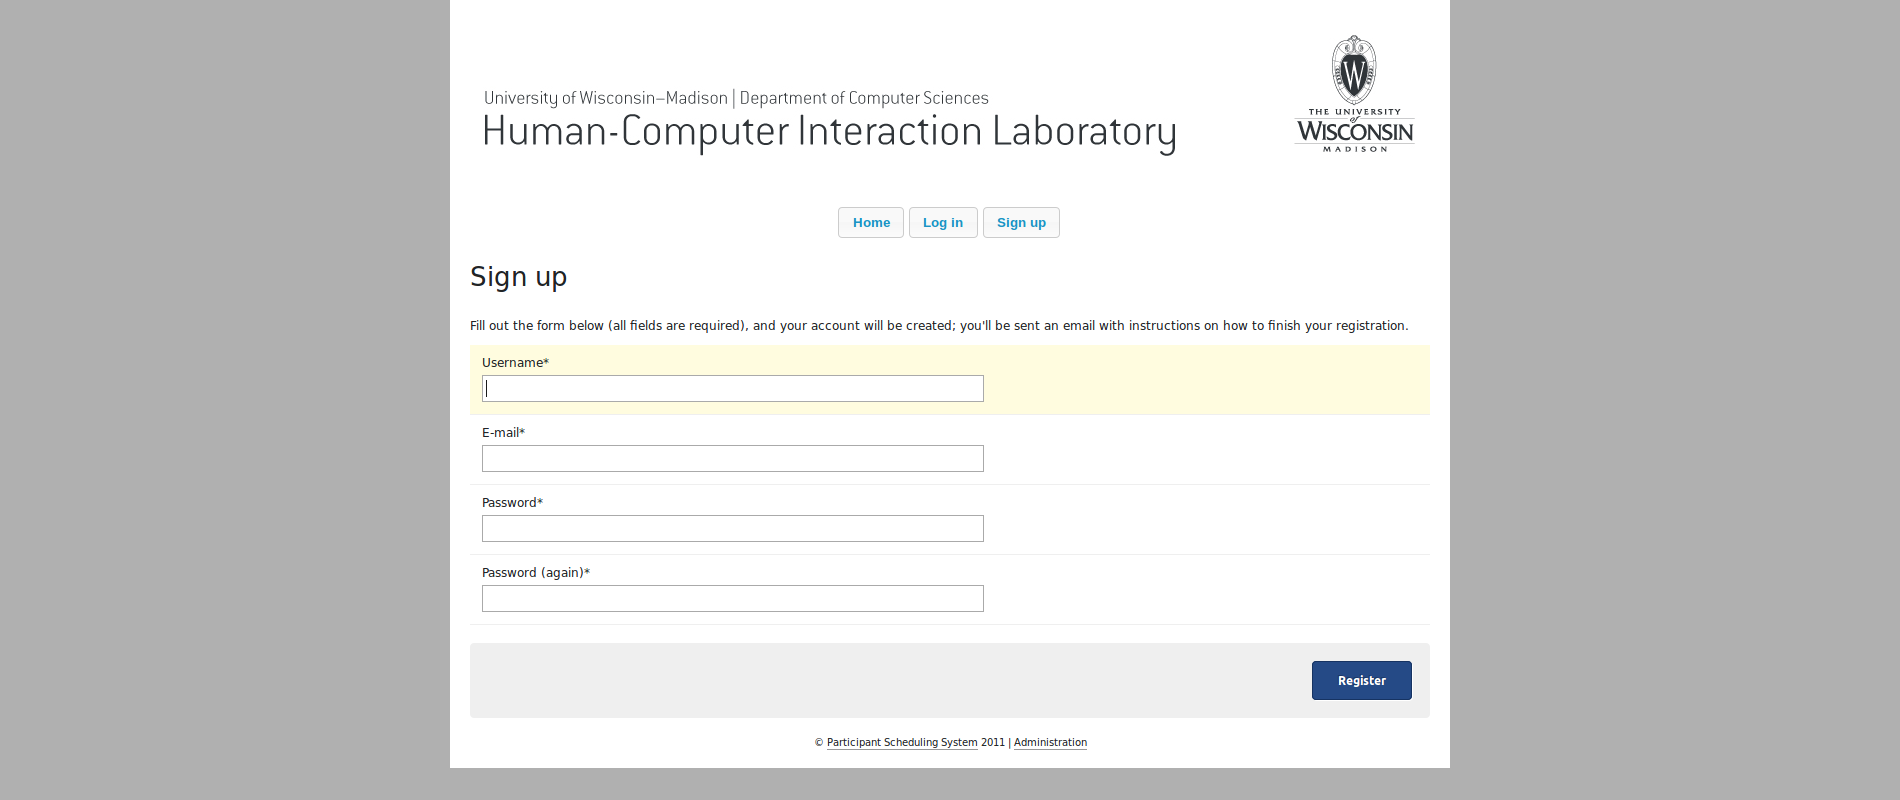
\includegraphics[width=6in]{../other/initial-interface-design/sign-up.png}
\subsubsection{Revised}
No changes

\subsection{Log In}
\subsubsection{Initial}
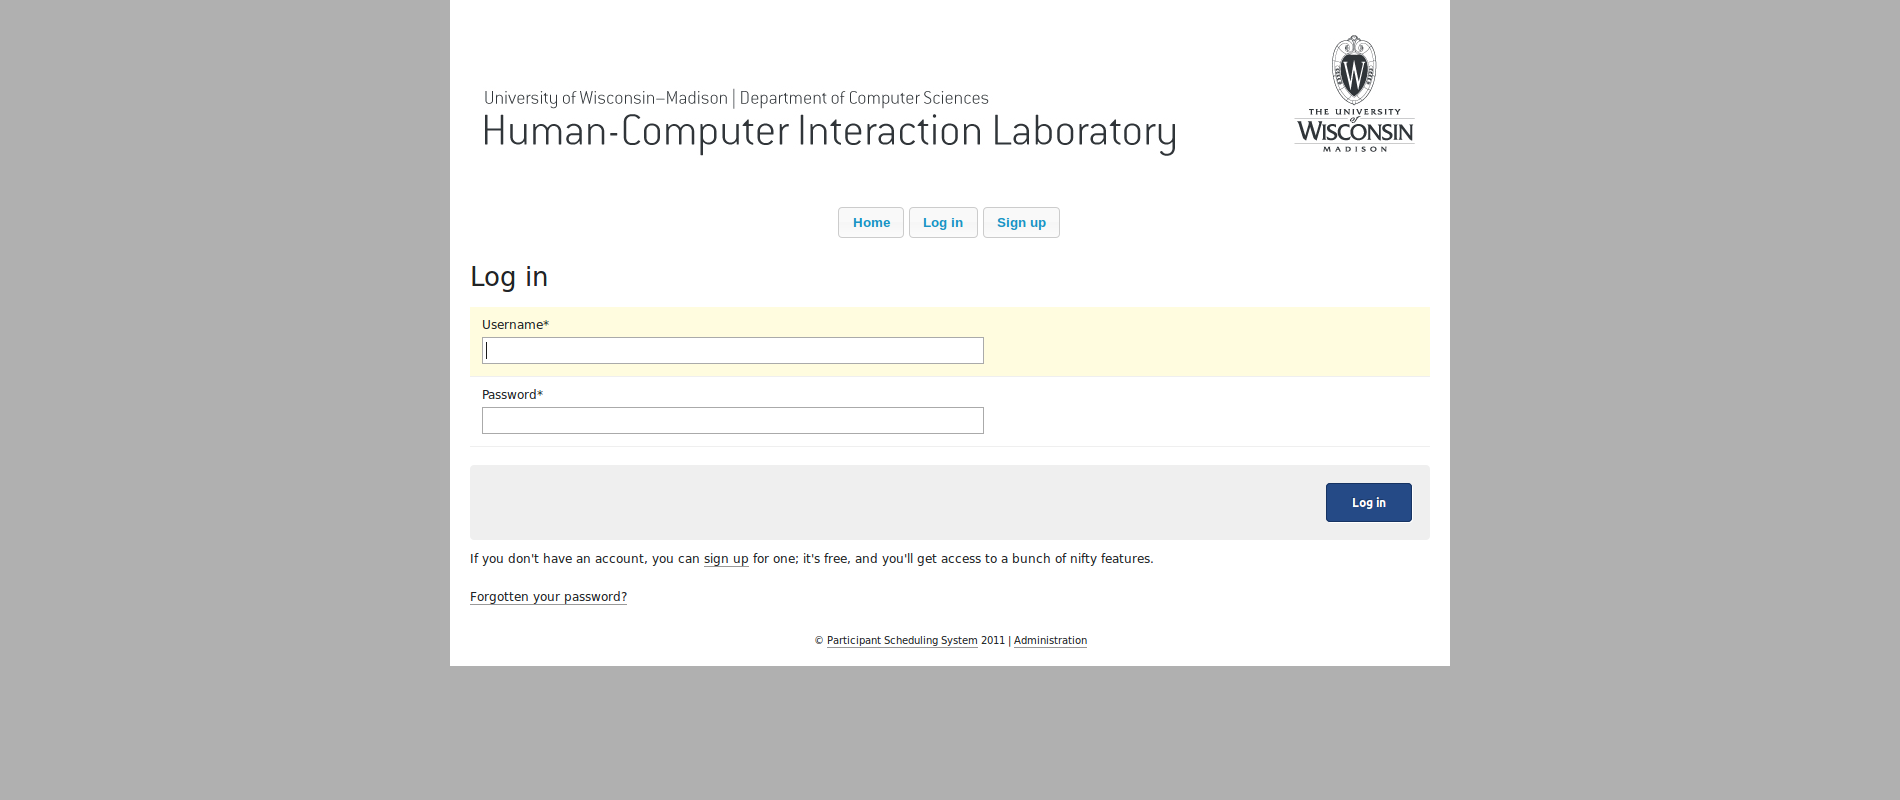
\includegraphics[width=6in]{../other/initial-interface-design/log-in.png}
\subsubsection{Revised}
No changes

\subsection{Password Reset}
\subsubsection{Initial}
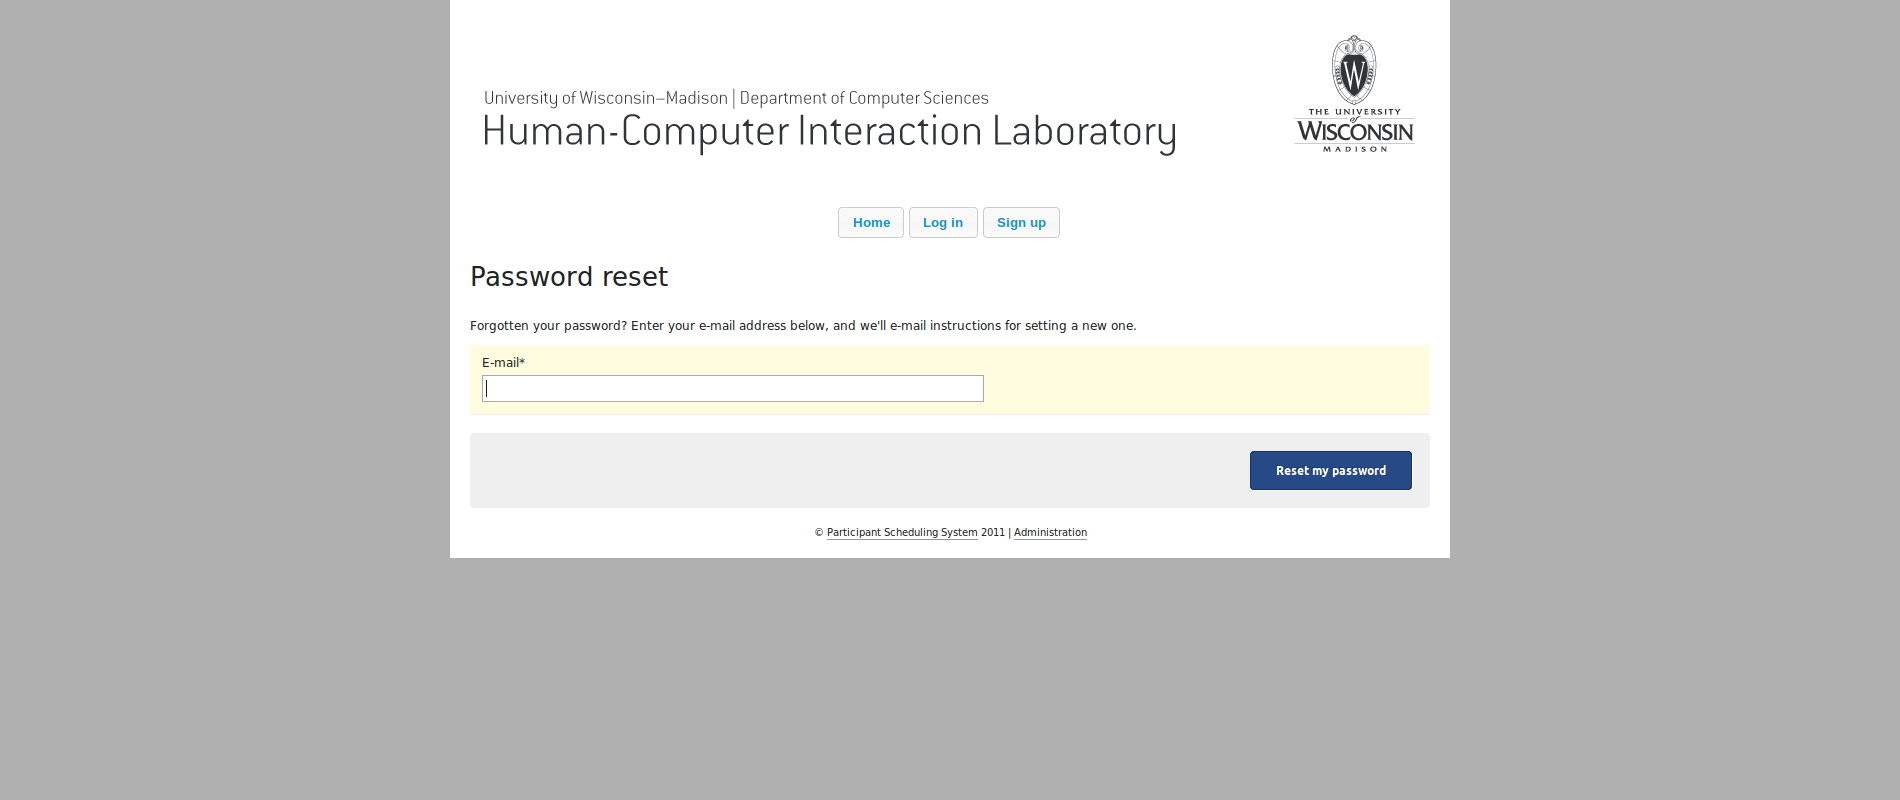
\includegraphics[width=6in]{../other/initial-interface-design/password-reset.png}
\subsubsection{Revised}
No changes

\subsection{Home, Logged In}
\subsubsection{Initial}

\includegraphics[width=6in]{../other/initial-interface-design/home-2.png}
\subsubsection{Revised}
Upon logging in, instead of being taken back to the home page, the user will be taken to the experiments page. If the user manually returns to the home page while logged in, the revisions of the default home page will be reflected there as well; see \textbf{Home, Logged In}. On every page, the logged in user's username or name will be displayed somewhere.

\subsection{Password Change}
\subsubsection{Initial}
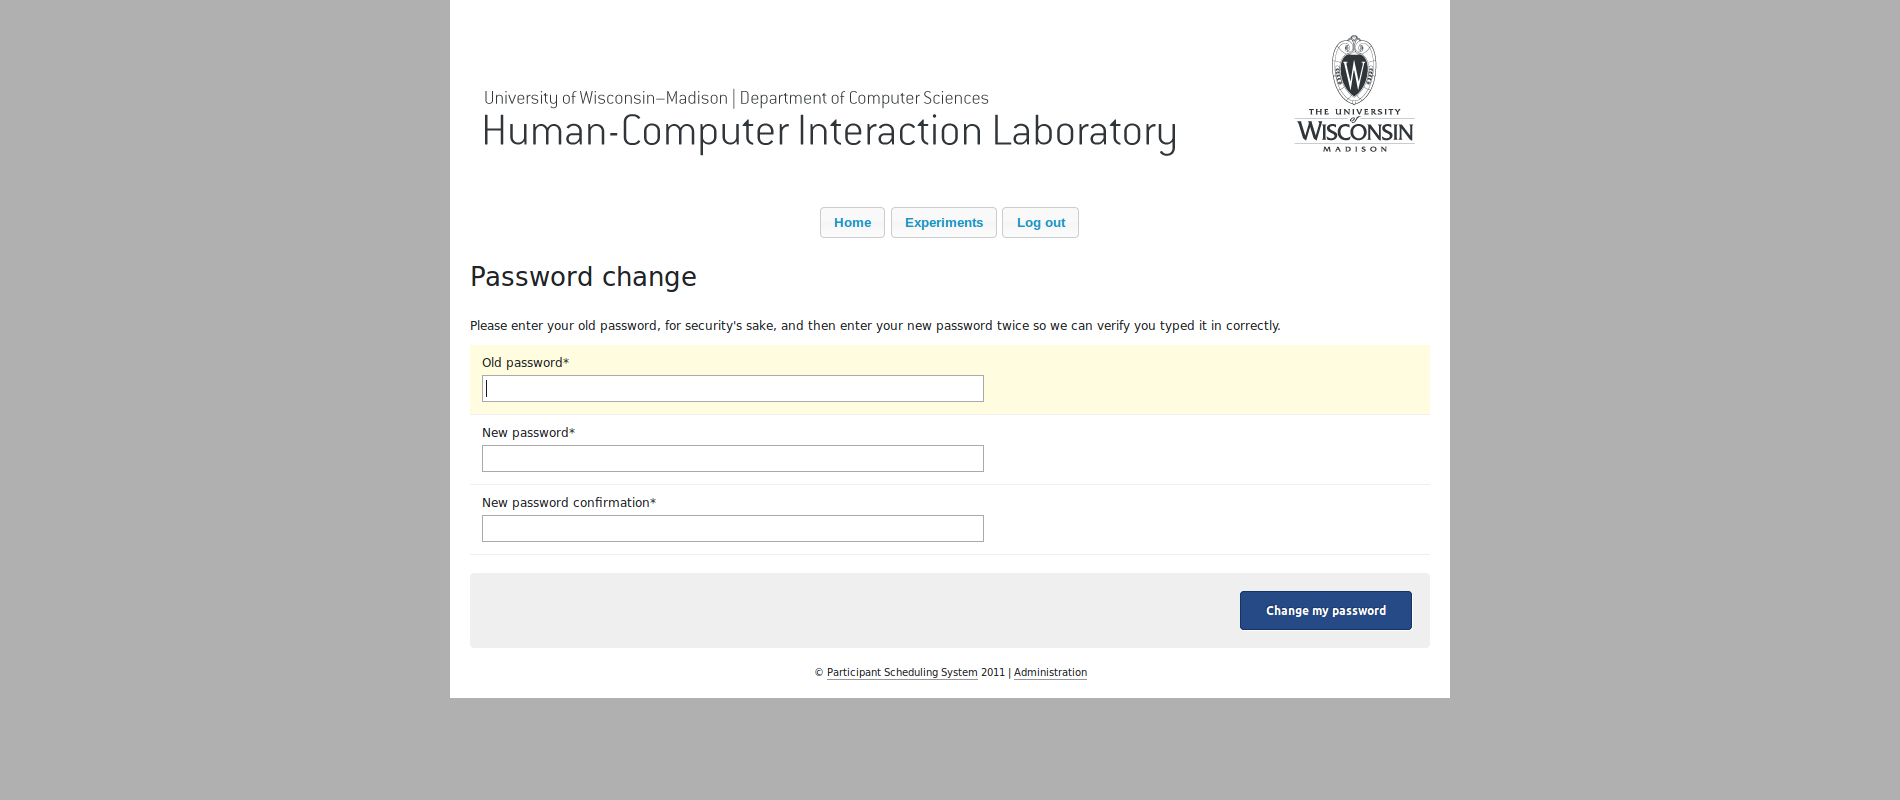
\includegraphics[width=6in]{../other/initial-interface-design/password-change.png}
\subsubsection{Revised}
It will be linked to from some other page, maybe the home page while logged in. No user was able to access it without explicitly visiting the URL, which they were not given.

\subsection{Experiments}
\subsubsection{Initial}
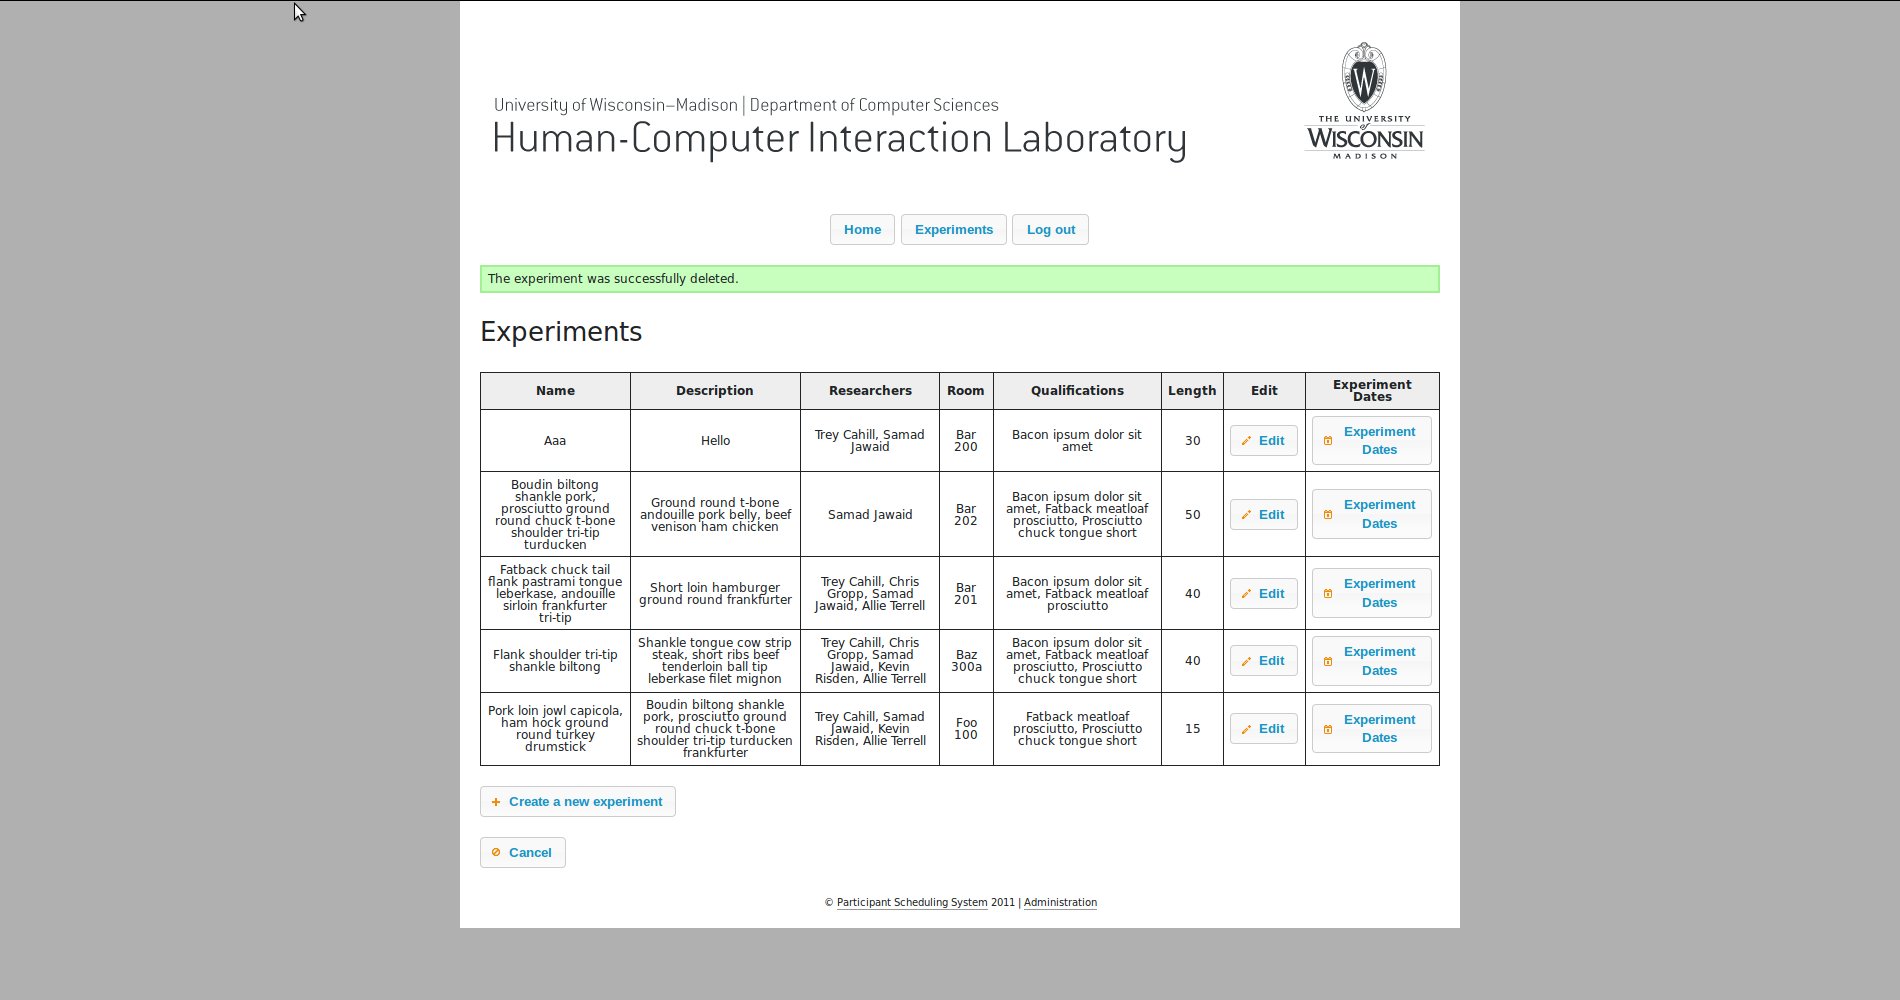
\includegraphics[width=6in]{../other/initial-interface-design/experiments.png}
\subsubsection{Revised}
The unit of length (minutes) will be specified. The table will be filterable and sortable. Experiments will be able to be mass-deleted from the table. The create button will be duplicated above the table as well. The cancel button will be changed to a back button with an appropriate icon.

\subsection{Create Experiment}
\subsubsection{Initial}
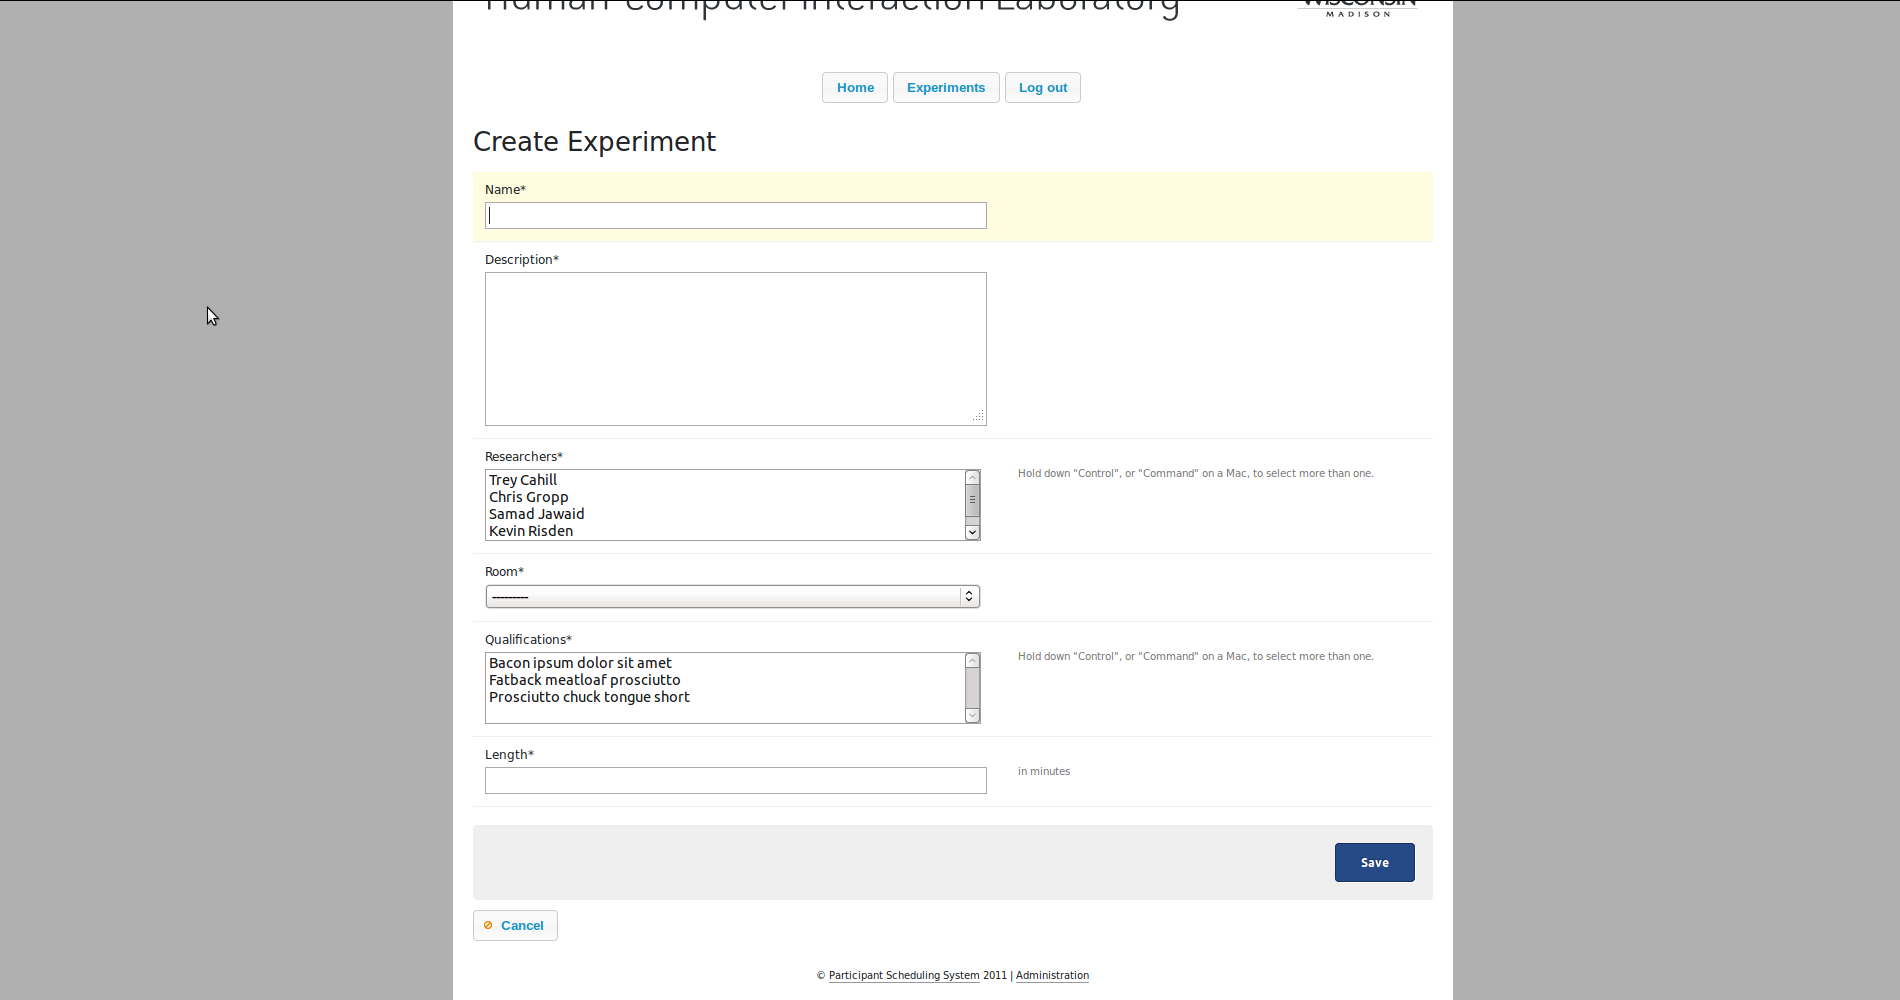
\includegraphics[width=6in]{../other/initial-interface-design/create-experiment.png}
\subsubsection{Revised}
The qualifications, room, and researchers inputs will be jQueryUI autocomplete fields with the ability to create new values. It will be clear that the cancel button discards all unsaved changes.

\subsection{Edit Experiment}
\subsubsection{Initial}
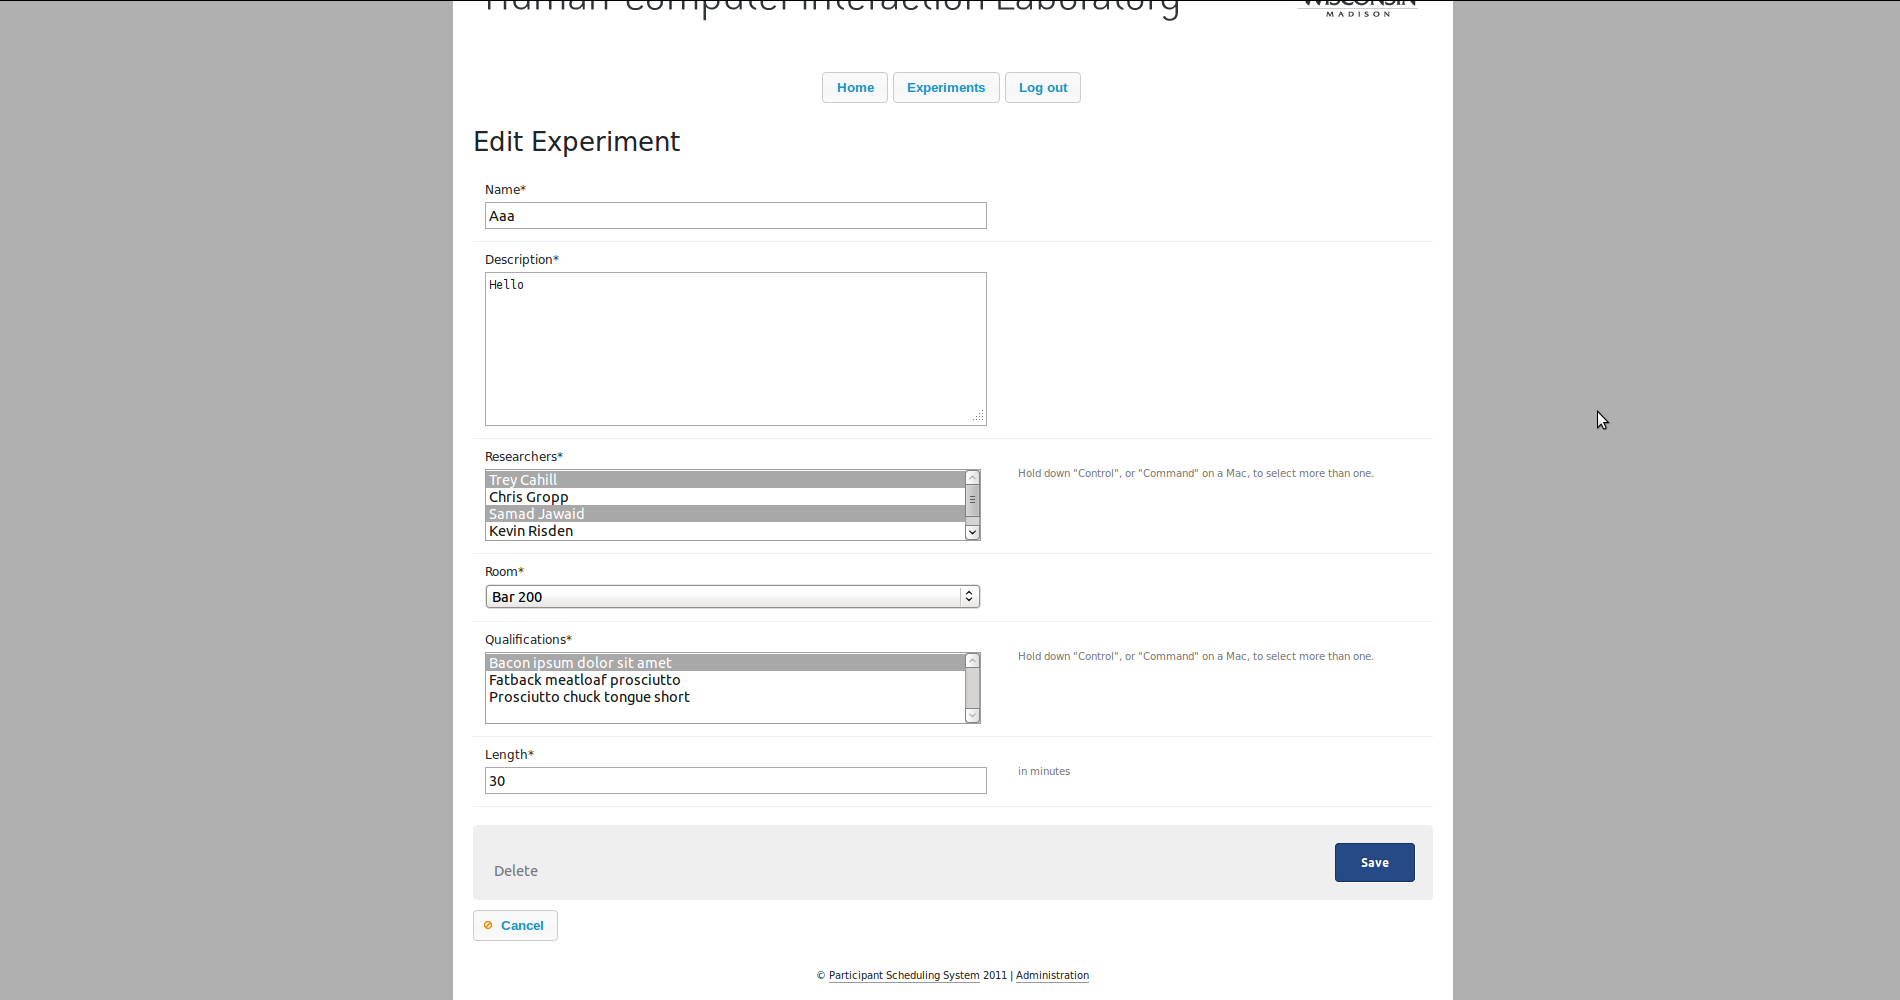
\includegraphics[width=6in]{../other/initial-interface-design/edit-experiment.png}
\subsubsection{Revised}
The delete button will not be so subtle. Also, see \textbf{Create Experiment}.

\subsection{Delete Experiment}
\subsubsection{Initial}
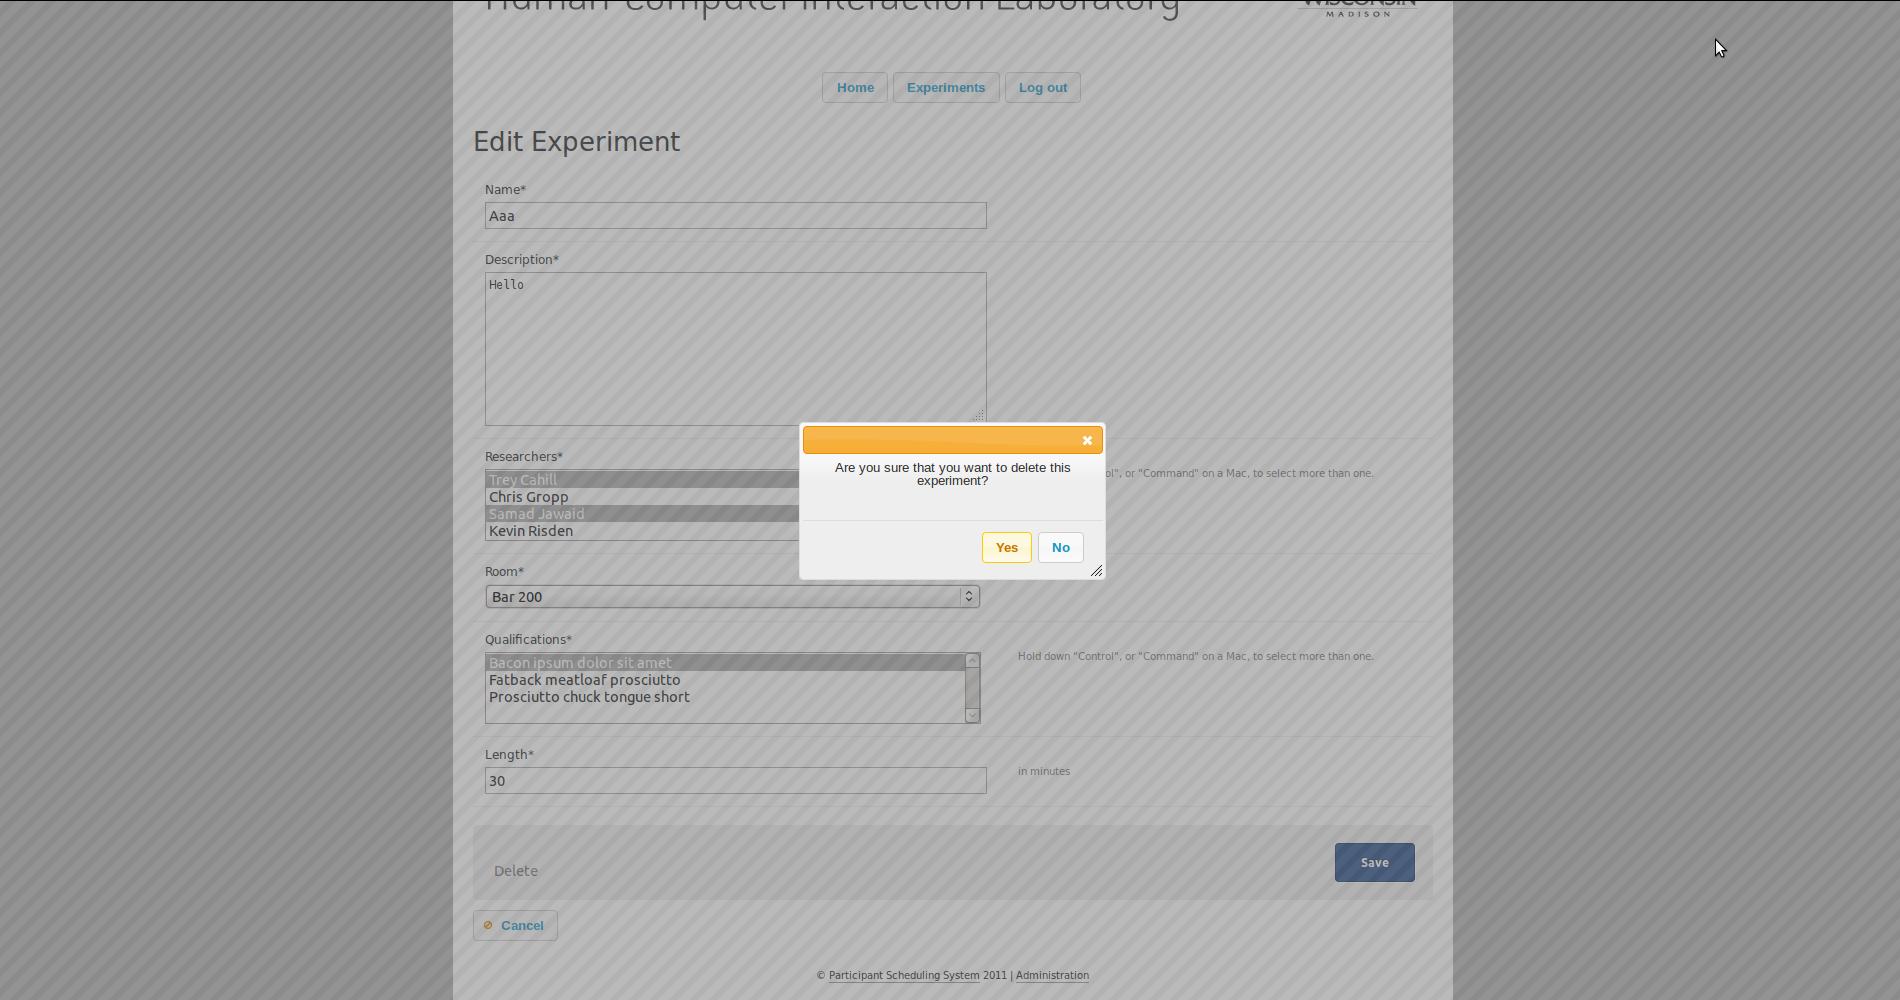
\includegraphics[width=6in]{../other/initial-interface-design/delete-experiment.png}
\subsubsection{Revised}
The jQueryUI CSS theme will match the existing CSS, so the dialog box will not appear so out of place.

\subsection{Experiment Dates}
\subsubsection{Initial}
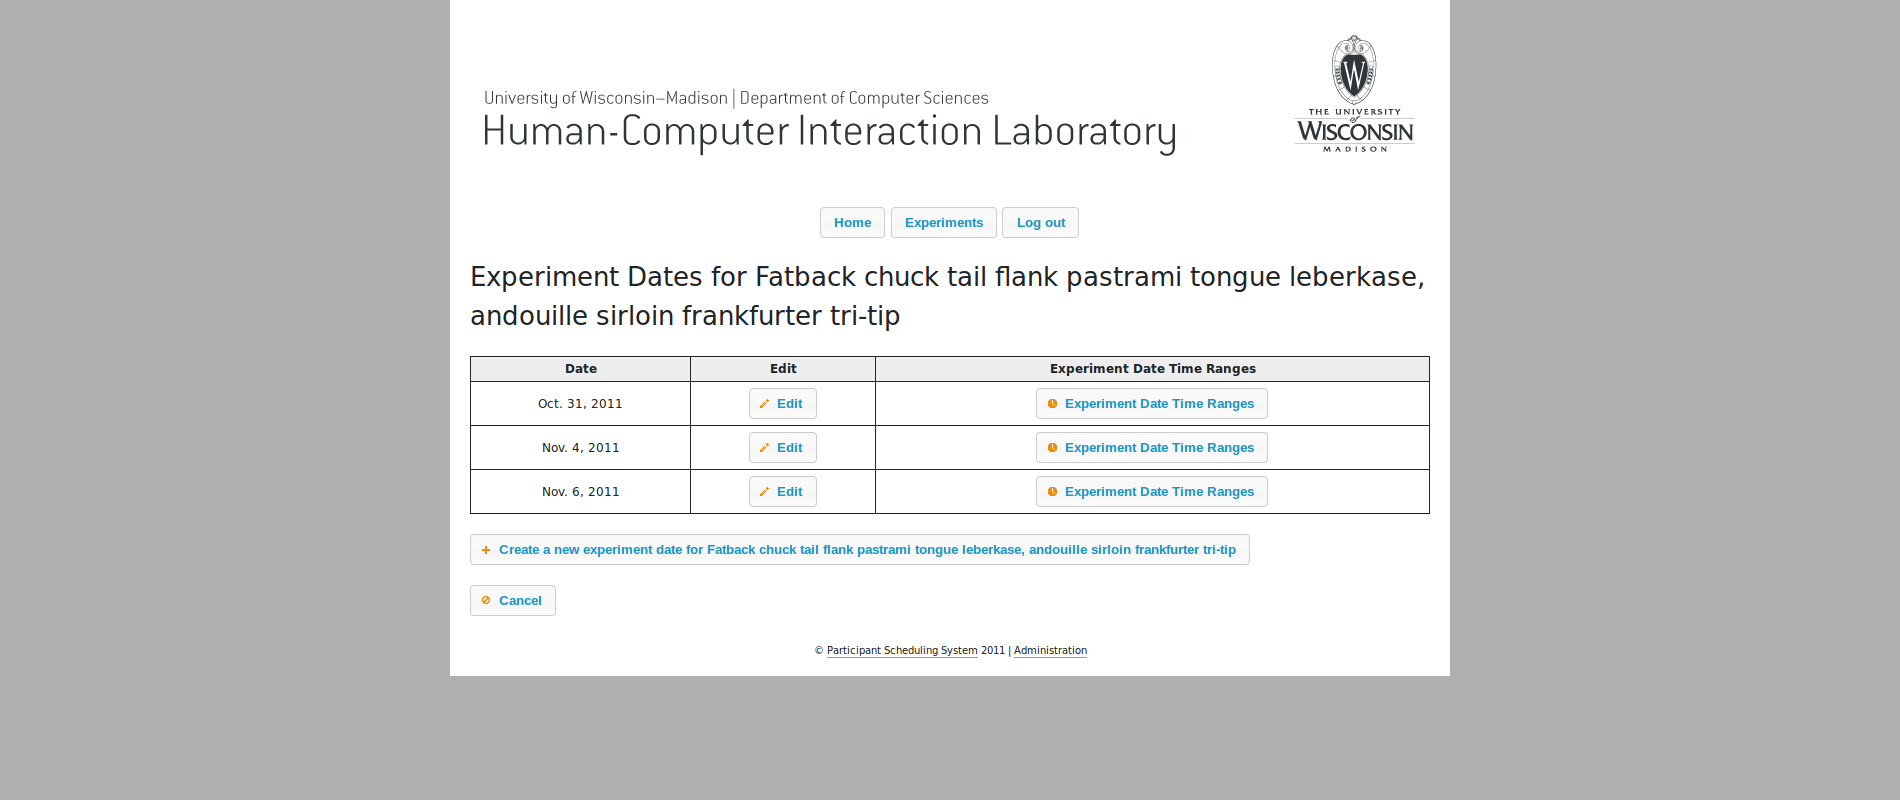
\includegraphics[width=6in]{../other/initial-interface-design/experiment-dates.png}
\subsubsection{Revised}
The table will be filterable and sortable. Experiment dates will be able to be mass-deleted from the table. The create button will be duplicated above the table as well. The cancel button will be changed to a back button with an appropriate icon.

\subsection{Create Experiment Date}
\subsubsection{Initial}
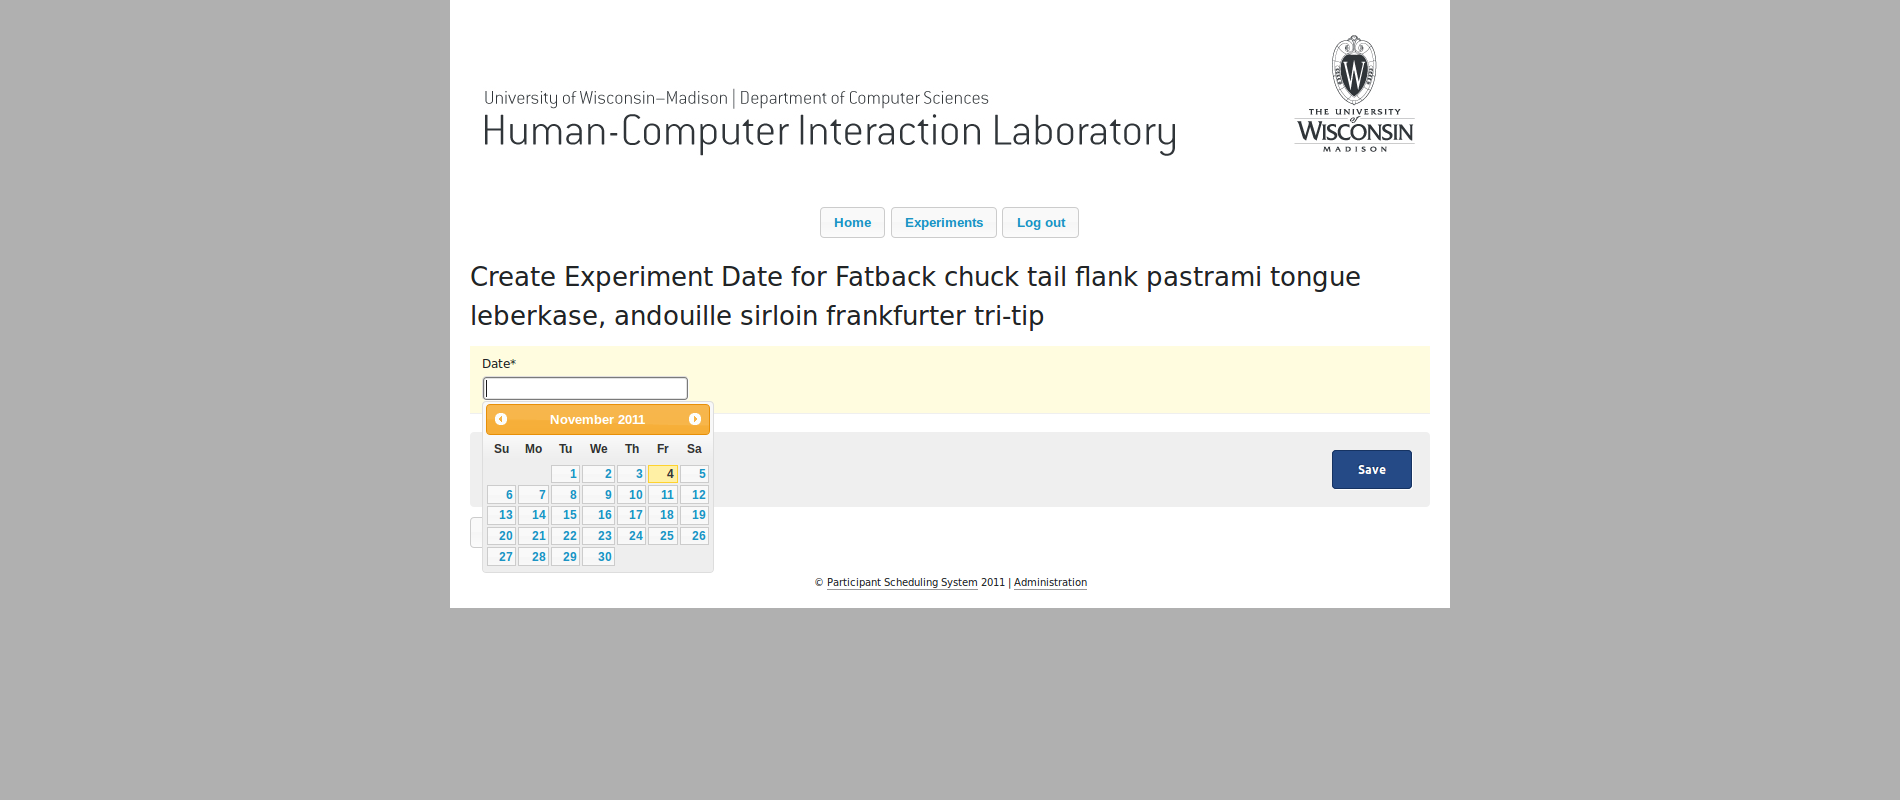
\includegraphics[width=6in]{../other/initial-interface-design/create-experiment-date.png}
\subsubsection{Revised}
The user will be able to type in a date manually without using the calendar widget. Help text explaining the date format will be added. The widget will not automatically appear on page load. It will be clear that the cancel button discards all unsaved changes.

\subsection{Edit Experiment Date}
\subsubsection{Initial}
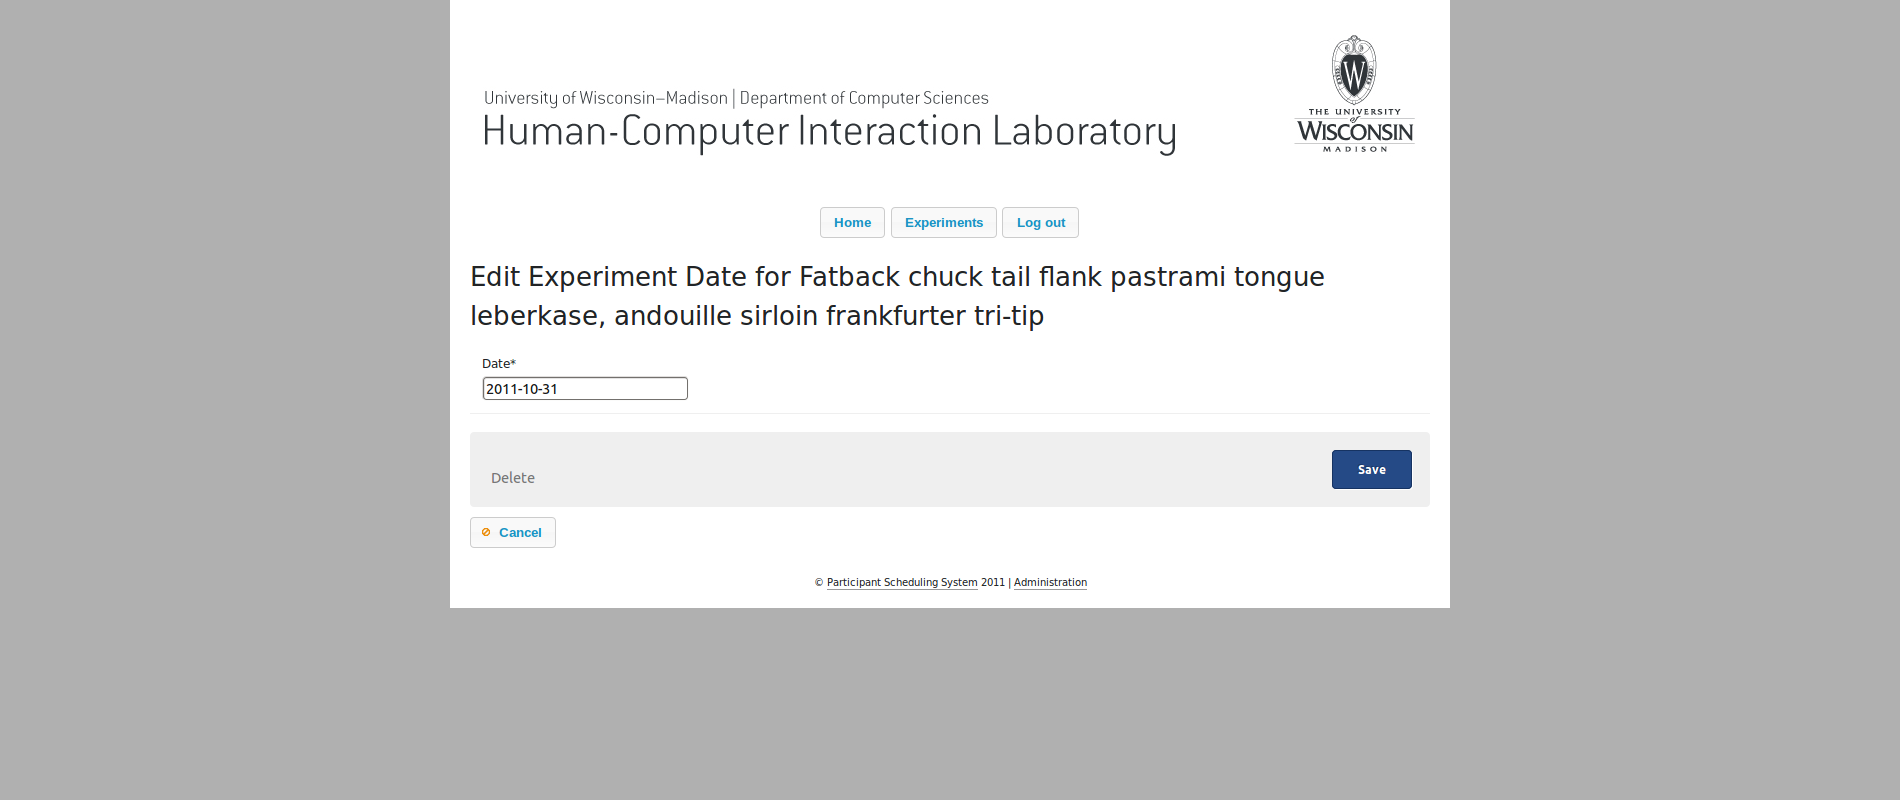
\includegraphics[width=6in]{../other/initial-interface-design/edit-experiment-date.png}
\subsubsection{Revised}
The delete button will not be so subtle. Also, see \textbf{Create Experiment Date}.

\subsection{Delete Experiment Date}
\subsubsection{Initial}
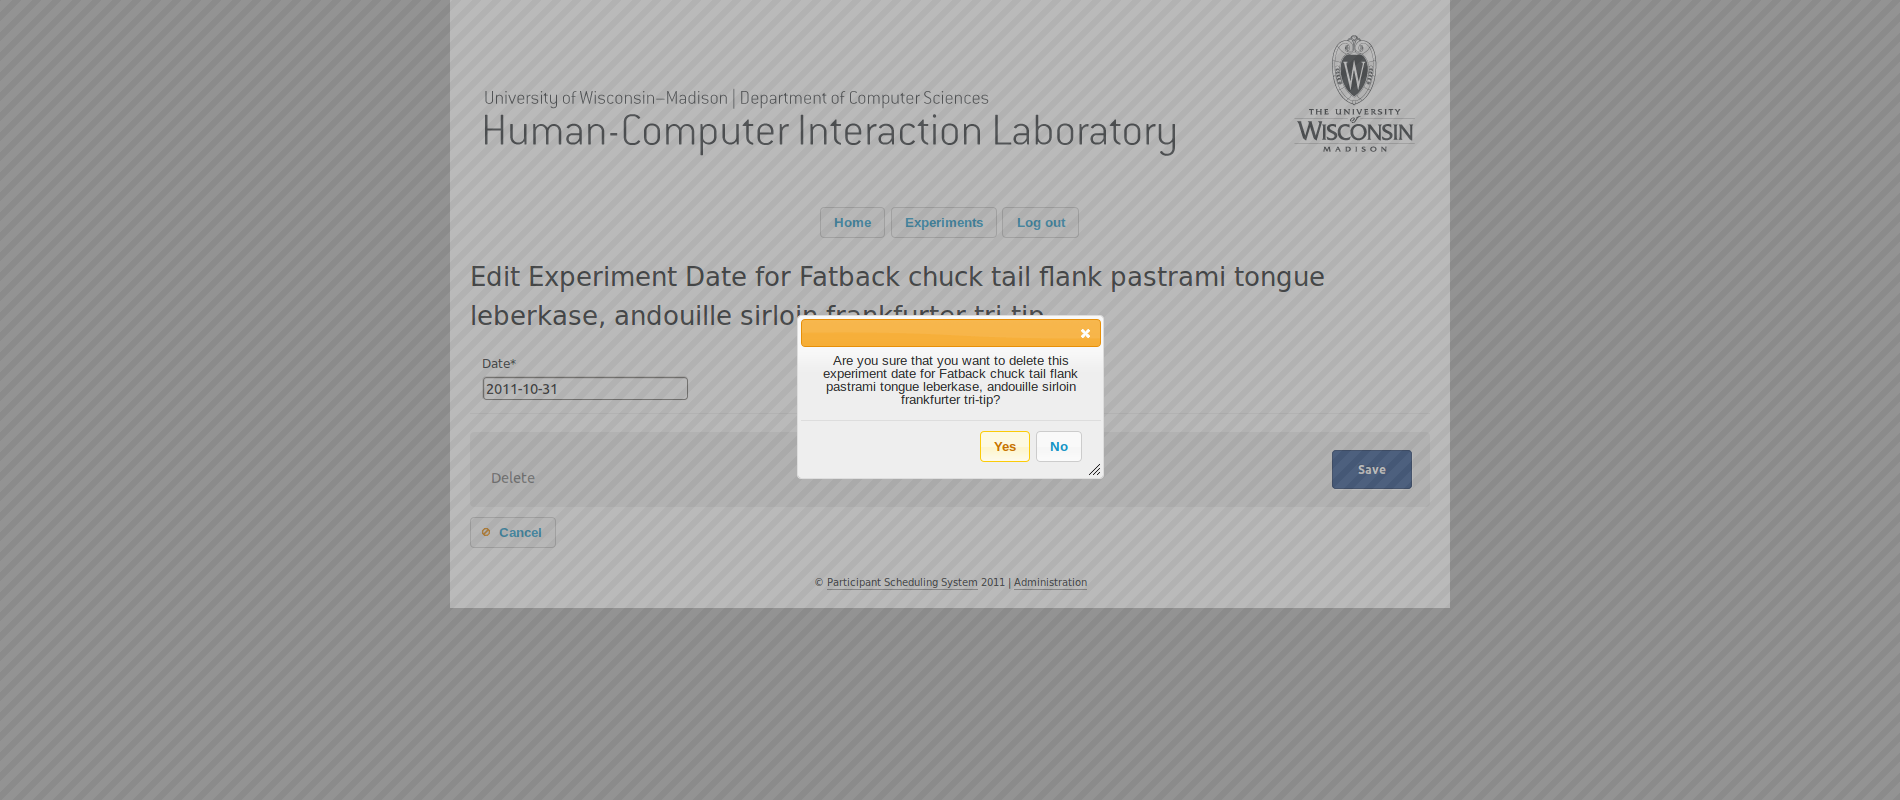
\includegraphics[width=6in]{../other/initial-interface-design/delete-experiment-date.png}
\subsubsection{Revised}
The jQueryUI CSS theme will match the existing CSS, so the dialog box will not appear so out of place.

\subsection{Experiment Date Time Ranges}
\subsubsection{Initial}
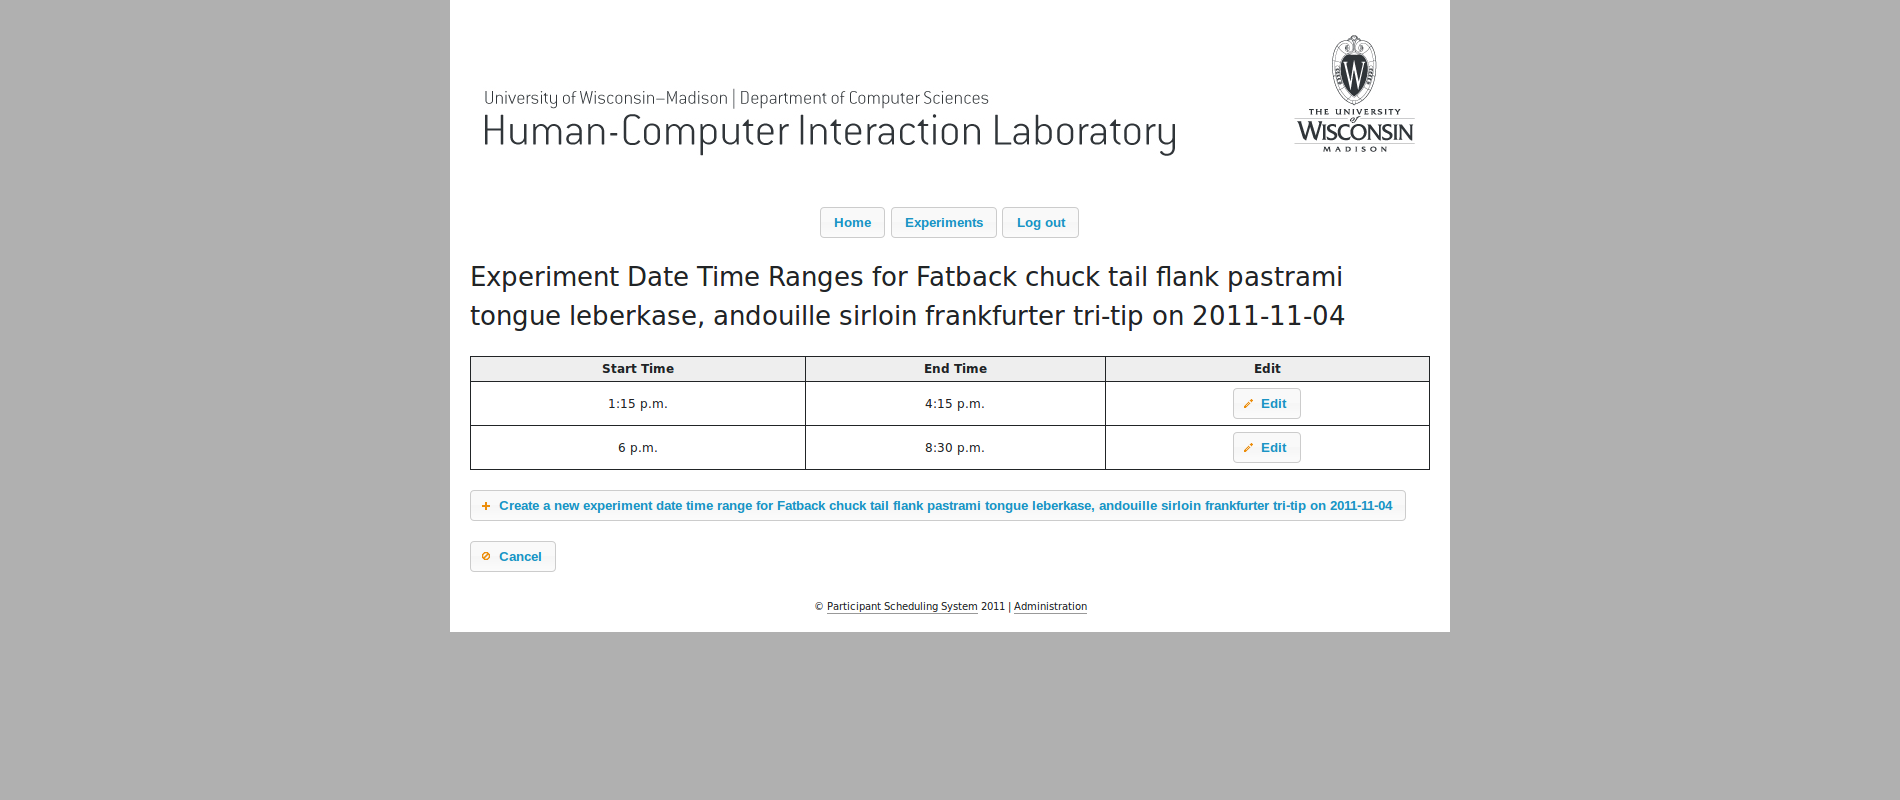
\includegraphics[width=6in]{../other/initial-interface-design/experiment-date-time-ranges.png}
\subsubsection{Revised}
The table will be filterable and sortable. Experiment date time ranges will be able to be mass-deleted from the table. The create button will be duplicated above the table as well. The cancel button will be changed to a back button with an appropriate icon.

\subsection{Create Experiment Date Time Range}
\subsubsection{Initial}
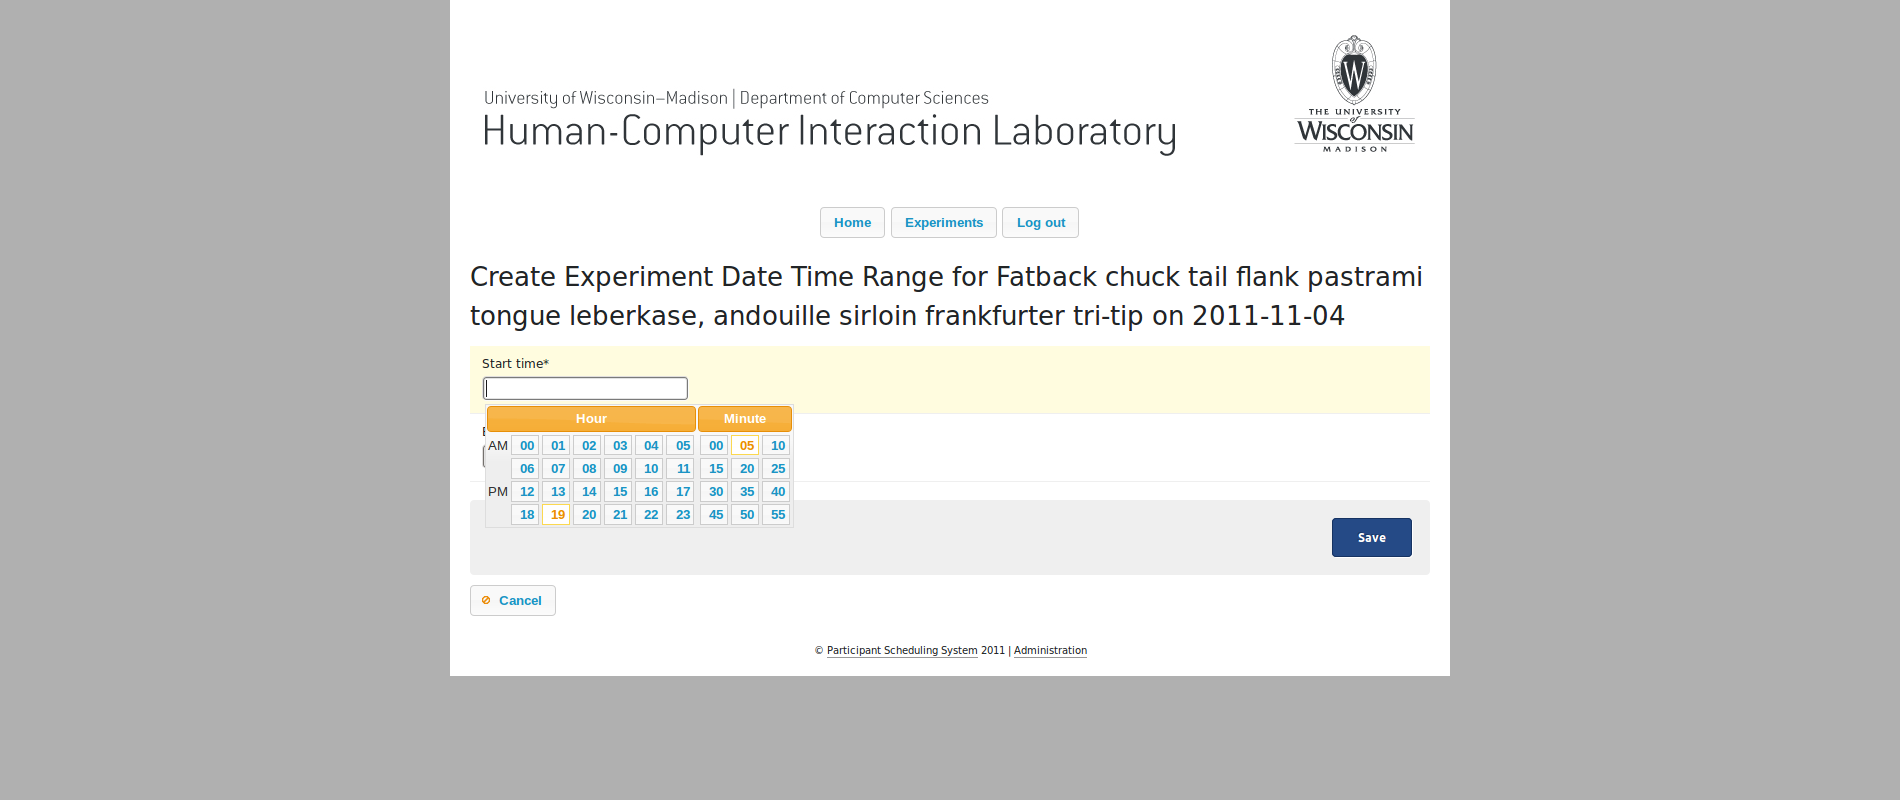
\includegraphics[width=6in]{../other/initial-interface-design/create-experiment-date-time-range.png}
\subsubsection{Revised}
The time widget will not have the AM or PM labels since it uses 24-hour time. Help text explaining the time format will be added. The widget will not automatically appear on page load. It will be clear that the cancel button discards all unsaved changes.

\subsection{Edit Experiment Date Time Range}
\subsubsection{Initial}
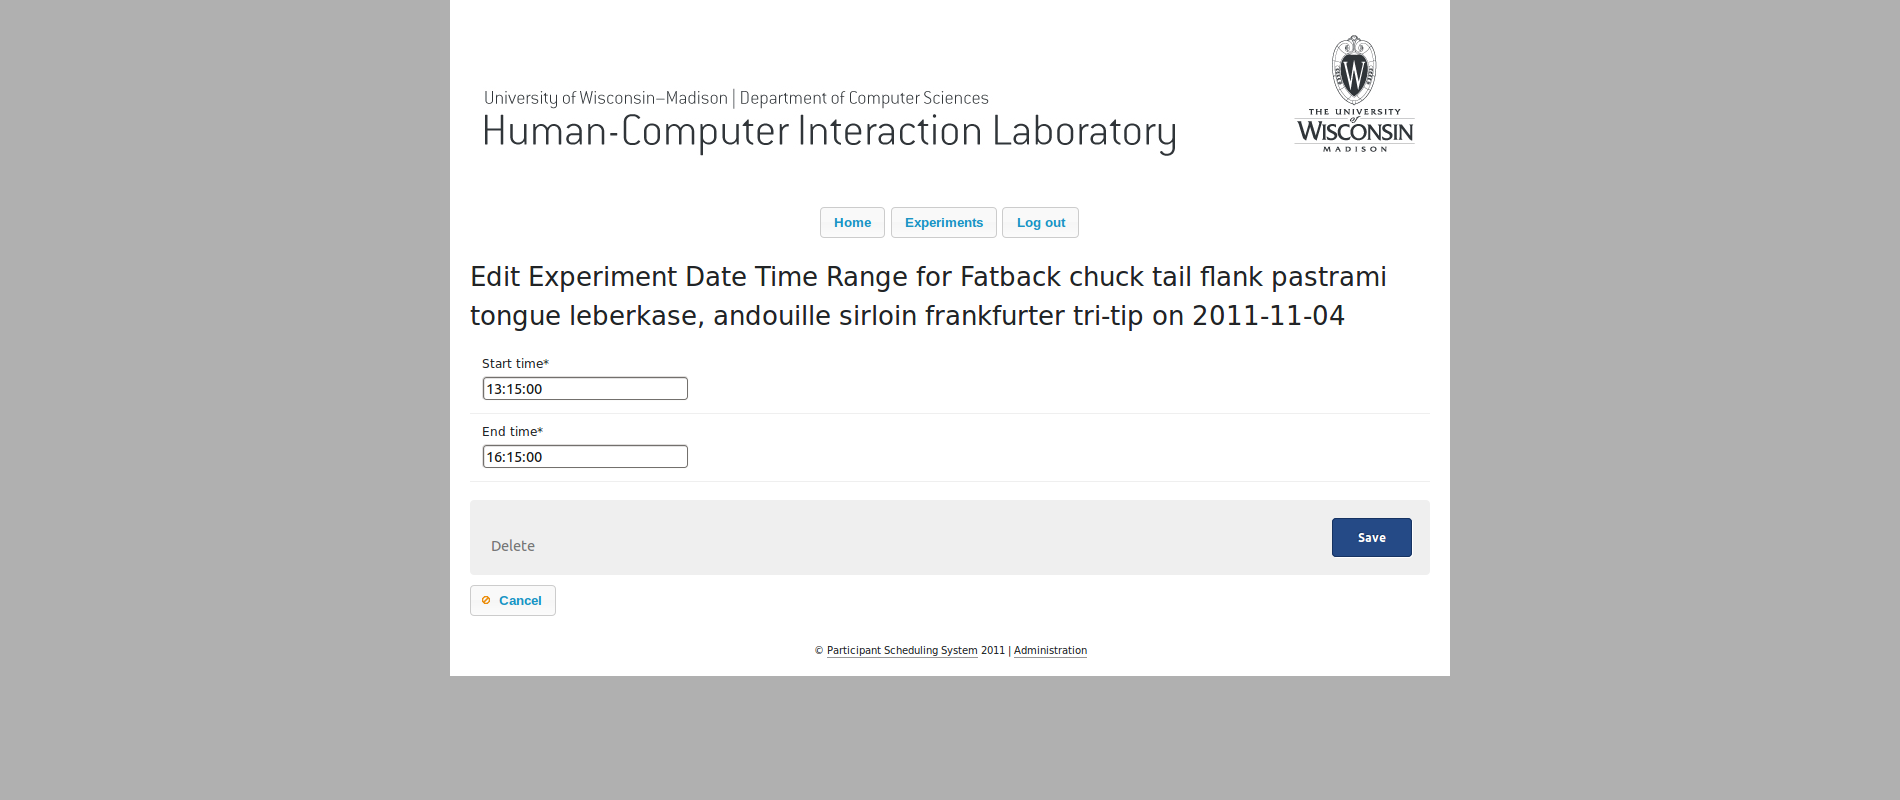
\includegraphics[width=6in]{../other/initial-interface-design/edit-experiment-date-time-range.png}
\subsubsection{Revised}
The delete button will not be so subtle. Also, see \textbf{Create Experiment Date Time Range}.

\subsection{Delete Experiment Date Time Range}
\subsubsection{Initial}
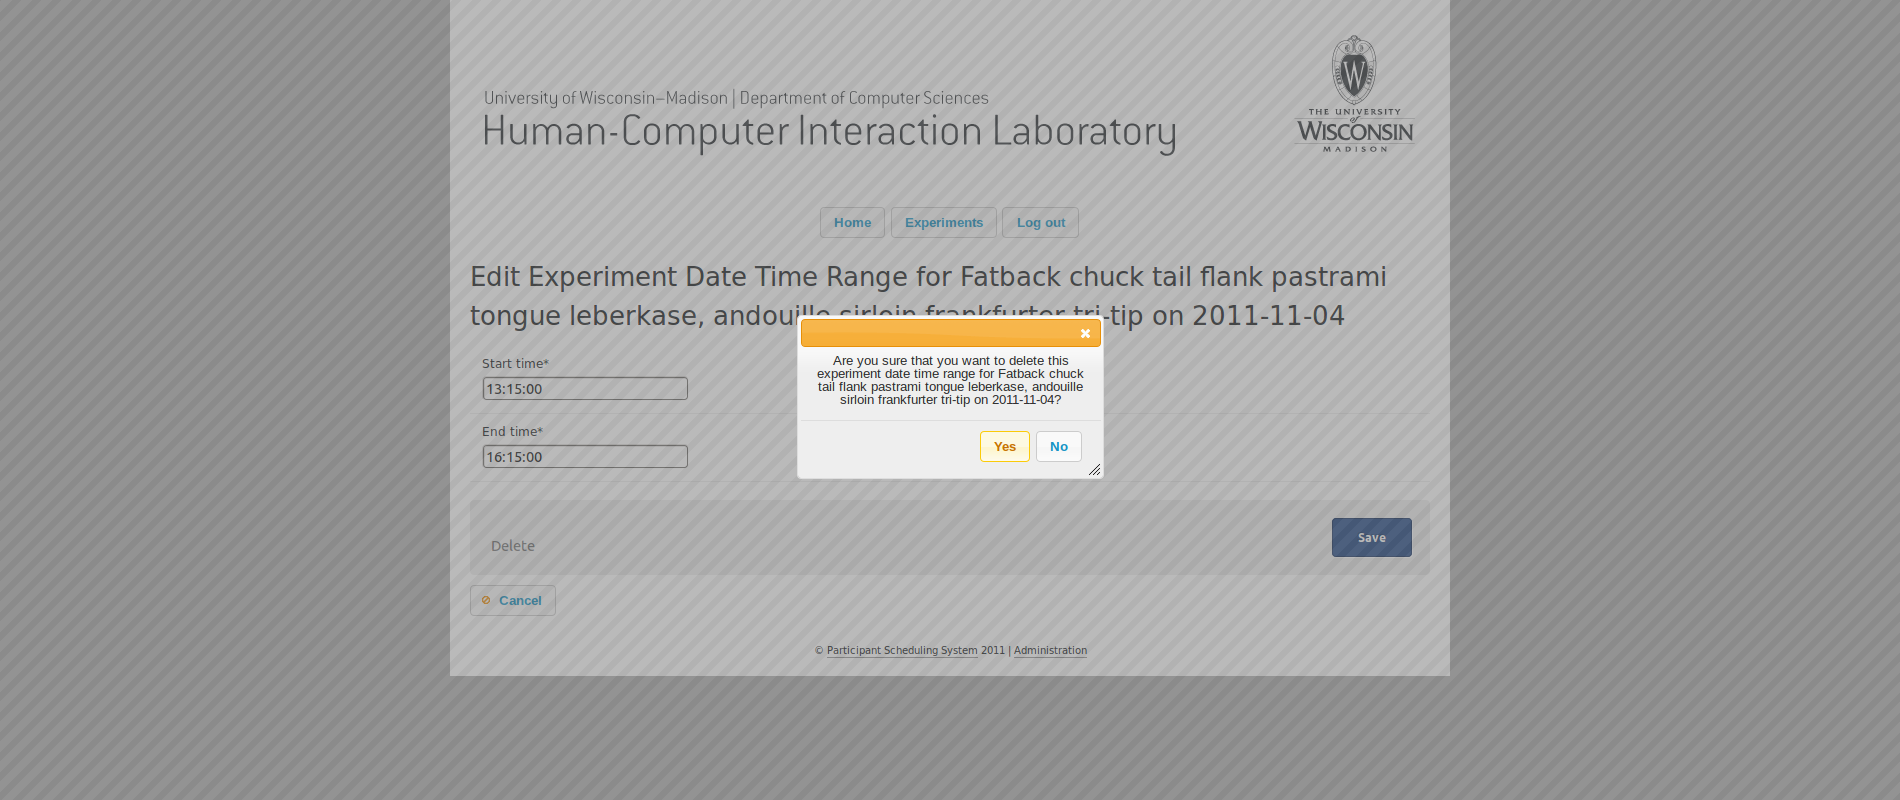
\includegraphics[width=6in]{../other/initial-interface-design/delete-experiment-date-time-range.png}
\subsubsection{Revised}
The jQueryUI CSS theme will match the existing CSS, so the dialog box will not appear so out of place.

% End - Milestone 5 specific parts
% fix for bibliography title
\renewcommand\refname{\section{References}}{\vspace*{-12mm}}
\bibliographystyle{plain}
\bibliography{bibliography}

\section{Appendix}

\section{Glossary}

\section{Index}

\end{document}
